\documentclass[12pt,onecolumn,a4paper]{article}
\usepackage[brazilian]{babel}
\usepackage[utf8]{inputenc}
\usepackage{hyperref}
\usepackage[pdftex]{graphicx}
\usepackage{wrapfig}
\usepackage{sidecap}
\usepackage[section]{placeins}
%\usepackage{amsmath}


\begin{document}

% Title page.
\begin{titlepage}

    % Title info.
    \title{
        \bf
        \Huge  USPGameDev \\
        \normalsize Grupo de Pesquisa e Desenvolvimento de Jogos da USP \\
        \LARGE Relatório
    }
    \author{Wilson Kazuo Mizutani}
    
    % Print title.
    \maketitle
    
    % No numbering on this page.
    \thispagestyle{empty}
    
\end{titlepage}


% Print table of contents.
\tableofcontents

% Page break.
\clearpage

% Make pages from now on have a header.
\pagestyle{myheadings}
\markright{\large USPGameDev - Relatório}

% O Giuliano pediu para fazer o relatório em duas partes, uma com explicações e outra com
% resultados (usando imagens). A primeira ele estimou umas 5 páginas, e, para a segunda, 20.

%%% Parte I: Explicações. %%%

\section{\LARGE O que é o USPGameDev?}

    \subsection{Definição e objetivos}
        O USPGameDev é um grupo de pesquisa e desenvolvimento de jogos da USP. Ele tem como meta
        criar um ambiente no qual membros da comunidade USP interessados na criação de jogos
        eletrônicos possam por em prática o que aprenderam em seus cursos e desenvolver suas
        próprias ideias. Além disso, o grupo visa aprender sobre práticas de gerenciamento de
        equipes e projetos, sobre processos de elaboração criativa de jogos e, também, adquirir
        familiaridade com as atuais ferramentas de desenvolvimento utilizadas na área.
    
    \subsection{Filosofia}
        O grupo procura adotar uma filosofia de {\it Software Livre} - permitindo que qualquer um
        tenha acesso a estudar, modificar e redistribuir aquilo que produzimos - e de {\it
        Portabilidade} - garantindo que aquilo que produzimos possa ser compatível com a maior parte
        possível dos sistemas operacionais e arquiteturas encontradas nos computadores modernos. É
        do interesse do grupo que o maior número possível de pessoas possam usufruir dos nossos
        resultados, sem restrições.
    
    \subsection{Atividades}
    \label{sec:atividades}
        A rotina usual do grupo consiste em reuniões presenciais, três vezes por semana, para
        discussão e trabalho. Ou seja, é nessas reuniões que ocorre o desenvolvimento dos projetos
        nos quais o grupo está envolvido, assim como eventuais debates sobre metas futuras e suas
        prioridades. No entanto, além dos projetos centrais, há outras atividades nas quais o grupo
        participa.
        
        A primeira delas é a realização de palestras informativas para divulgar o trabalho do grupo
        e compartilhar experiências. Desde o seu primeiro lançamento, o grupo tem se esforçado para
        encontrar seu lugar na comunidade USP, realizando essas apresentações inclusive no campus da
        Escola de Artes, Ciências e Humanidades da USP.
        
        Outra atividade é o oferecimento de cursos técnicos, também voltados ao público da USP. A
        primeira bateria deles ocorreu durantes os meses de Outubro e Novembro de 2011. A intenção
        do grupo é oferer quatro cursos por semestre. O conteúdo deles abrange ferramentas de
        desenvolvimento de software como:

        \begin{itemize}
        
            \item{\bf CMake \footnotemark} - gerenciador de construção de projetos de software
                                             multiplataforma;
            \footnotetext{Site oficial: \url{www.cmake.org}}
            
            \item {\bf Lua \footnotemark} - linguagem de script brasileira muito usada por jogos de
                                            renome no mercado; e
            \footnotetext{Site oficial: \url{www.lua.org}}

            \item {\bf LÖVE \footnotemark} - uma plataforma para desenvolvimento de jogos em duas
                                             dimensões minimal e gratuita.
            \footnotetext{Site oficial: \url{www.love2d.org}}
            
        \end{itemize}
        
        Mas também aborda ferramentas de propósito mais geral como:
        
        \begin{itemize}
        
            \item {\bf Git \footnotemark} - ferramenta de controle de versão de projetos;
            \footnotetext{Site oficial: \url{www.git-scm.com}}
            
            \item {\bf \LaTeX \footnotemark} - programa de formatação de texto muito utilizado no
                                               mundo acadêmico; e
            \footnotetext{Site oficial: \url{www.latex-project.org}}
            
            \item {\bf SSH \footnotemark} - protocolo de rede que permite conexões seguras entre
                                            computadores.
            \footnotetext{Informações
                sobre: \url{pt.wikipedia.org/wiki/SSH};
                Site oficial: \url{http://www.ssh.com}
            }
        
        \end{itemize}
        
        Houve também um processo seletivo de novos membros que envolveu a confecção de quatro
        mini-projetos por parte dos candidatos. Tendo sido orientados pelo membros veteranos do
        grupo durante o processo, esses candidatos puderam adquirir uma experiência breve porém real
        de como é desenvolver um jogo, independentemente de terem sido posteriormente admitidos como
        membros ou não.
        
        Além dessas atividades, alguns integrantes do grupo ainda se organizam para participar de
        competições de desenvolvimento de jogos eletrônicos de tempos em tempos.
        
        Com o objetivo de divulgar tudo isso, o grupo criou um site. Nele todas as principais
        informações sobre essas atividades podem ser encontradas, dentre outras. Em particular, o
        site disponibiliza a documentação oficial dos projetos que o grupo realiza. O endereço do
        dito site é:
        
        \begin{center}
            \footnotesize
            \url{http://www.uspgamedev.org}
        \end{center}
    
    \subsection{Metodologia}
    \label{sec:metodologia}
        Para gerenciar as atividades do grupo, é seguida uma metodologia de trabalho derivada do
        {\it Scrum}. Um dos membros do grupo fez como Trabalho de Conclusão de Curso no Bacharelado
        em Ciência da Computação justamente analisando sobre como {\it Scrum} poderia ser aplicado à
        equipes de desenvolvimento de jogos, e usou o USPGameDev como caso de estudo. Portanto, para
        maiores detalhes sobre como a nossa metodologia funciona, recomenda-se a leitura da
        monografia resultante desse trabalho, que pode ser encontrada em:
        
        \begin{center}
            \footnotesize
            \url{http://www.linux.ime.usp.br/~vkdaros/mac499/files/scrum_for_games.pdf}
        \end{center}

\section{\LARGE Histórico}
    
    \subsection{O Começo \\ {\small(Novembro/2009 - Janeiro/2010)}}
        Em novembro de de 2009, o orientador pedagógico da Escola Politécnica (Poli), Giuliano
        Salcas Olguin, incentivou tanto alunos do Instituto de Matemática e Estatísitca (IME) quanto
        da Poli interessados em desenvolver jogos eletrônicos a se juntar e tentar criar um projeto.
        Assim, realizou-se a primeira reunião de interessados, contando com a presença de alunos do
        Bacharelado em Ciência da Computação e de Engenharia da Computação. Nessa mesma reunião
        surgiu a proposta para o primeiro jogo que o grupo tentaria construir, porém apenas seu
        gênero estava definido. Ainda não possuia nome nem temática.

        A partir de então, mantiveram-se encontros semanais para discutir idéias e elaborar mais
        sobre o primeiro projeto. Essa fase inicial foi bem complicada, e muitos dos membros
        iniciais acabaram desistindo. Mas os que permaneceram chegaram a um acordo e finalizaram uma
        proposta completa para o primeiro projeto: \textit{\textbf{Horus Eye}}. Um \textit{Game
        Design Document}\footnotemark foi escrito para orientar os desenvolvedores na produção do
        jogo em janeiro do ano seguinte.
        
        Nesse período, as reuniões semanais aconteciam tanto no Biênio quanto no IME.
        
        \footnotetext{
            Infelizmente, a versão original do documento está em um site com acesso restrito. Uma
            versão alternativa pode ser encontrada na wiki do grupo (ver site oficial).
            
            Mais informações sobre \textit{Game Design Document}:
            
            \url{http://en.wikipedia.org/wiki/Game\_design\_document}
        }

    \subsection{Primeira fase de desenvolvimento do \textit{\textbf{Horus Eye}} \\
                {\small(Fevereiro/2010 - Setembro/2010)} }
        Com a ideia do jogo bem formada, o grupo deu início ao seu desenvolvimento. Pelas
        ferramentas escolhidas serem de baixo nível (veja a seção \ref{sec:horus}) o processo
        inicial foi trabalhoso e não apresentava quase nenhum resultado visual. O primeiro deles foi
        aparecer só depois de dois meses de esforço, embora por trás houvesse um ferramental bem
        maior já funcionando.
        
        Uma vez começado o semestre letivo, as reuniões voltaram à sua frequência usual. Dessa vez,
        a maior parte delas ocorria no Biênio.
        
        As funcionalidades necessárias ao jogo foram sendo implantadas ao longo do semestre. Nesse
        período alguns membros novos ingressaram no projeto para ajudarem com a arte gráfica. Nem
        todos eles ficaram até o fim, mas o jogo já tinha a maior parte da aparência atual pelo
        final do semestre. Com isso, o crescimento do jogo aumentou drasticamente no mês de Julho,
        uma vez que agora a arquitetura básica dele estava bem estabelecida.
        
        Embora não se pudesse chamar o \textit{\textbf{Horus Eye}} de um jogo \textit{completo},
        todos os requisitos exigidos pelo \textit{Game Design Document} haviam sido satisfeitos. Os
        meses de Agosto e Setembro compuseram uma fase de revisões e melhoramentos.

    \subsection{Lançamento do \textit{\textbf{Horus Eye}} e novas metas \\
                {\small(Outubro/2010 - Novembro/2010)} }
        Em Outubro de 2010, o \textit{\textbf{Horus Eye}} foi oficialmente lançado pelo grupo. O
        lançamento foi feito em uma apresentação no IME, embora as reuniões continuassem
        sendo realizadas majoritariamente no Biênio. Pouco tempo depois ocorreu também o lançamento
        do site do grupo (que na época tinha apenas algumas páginas e o fórum).
        
        Com o primeiro grande passo dado, o grupo passou rever os objetivos. Após alguma discussões,
        o que ficou decidido foi que o grupo precisava: recrutar novos membros, começar um novo
        projeto, e melhorar o suporte gráfico do \textit{\textbf{Horus Eye}}. Houve algumas
        propostas para o próximo jogo, mas nada ficou definido naquela época. O projeto de melhoria
        no \textit{\textbf{Horus Eye}} havia começado mas levaria ainda mais alguns meses para ser
        concluído. O processo seletivo que seria usado no recrutamento dos novos membros, no
        entanto, fora planejado e posto em prática logo em seguida.

    \subsection{Processo seletivo de novos membros \\
                {\small(Novembro/2010 - Abril/2011)} }
        Apesar de não ter sido a intenção original, a maior parte da atenção do grupo nesse período
        se focou no processo seletivo. Havia um total de aproximadamente setenta candidatos, e
        gerenciar a presença e a participação deles exigiu tempo e cuidado. Ao final foram
        selecionados dezoito novos membros, que incluíam dessa vez alunos não só do IME, da Poli, e
        da FAU, como também da Escola de Comunicação e Artes (ECA) e da Faculdade de Filosofia,
        Letras, e Ciências Humanas (FFLCH).
        
        Um dos principais resultados do processo seletivo foram os mini-projetos realizados pelos
        candidatos, como explicado na seção \ref{sec:atividades}. E nesse meio tempo, a migração de
        sistema gráfico do \textit{\textbf{Horus Eye}} foi finalizada. As propostas de separar mais
        claramente o jogo da \textit{framework} direcionavam o grupo à criação da \textbf{UGDK}.
        
        No dia 29 de Abril, alguns membros deram uma palestra sobre o grupo no campus da EACH.

    \subsection{Escolha e elaboração de um segundo projeto \\
                {\small(Maio/2011 - Junho/2011)} }
        Terminado o processo seletivo, o grupo agora dispunha de um maior arsenal de mentes
        criativas e capazes para desenvolver jogos. As discussões para o segundo projeto foram
        retomadas. Esse processo levou entre um e dois meses até que se houvesse decidido qual seria
        o novo jogo, seu gênero e sua temática.
        
        Em seguida foi decidida qual a ferramenta de desenvolvimento que seria usada. Como explicado
        na seção \ref{sec:pirates}, dessa vez se desejava uma ferramenta de alto nível, para que o
        projeto evoluísse mais rapidamente. E também se passaria a usar uma nova metodologia de
        trabalho.
        
        Nessa época, o grupo sofreu com algumas dificuldades em encontrar um lugar fixo para suas
        reuniões, visto que a sala que normalmente usavam no Biênio estava em reforma.

    \subsection{\textit{Scrum}, cursos e novos lançamentos \\
                {\small(Julho/2011 - Dezembro/2011)} }
        A metologia baseada em \textit{Scrum} mencionada na seção \ref{sec:metodologia} tem sido
        utilizada pelo grupo desde o início do segundo projeto. Antes disso, o grupo não seguia
        nenhuma metodologia em particular. Com essa nova maneira de trabalhar, ficou mais fácil de
        medir e documentar a produtividade do grupo.
        
        Mas além do novo projeto e do novo esquema de trabalho, foi nesse período que o grupo também
        deu início aos cursos (listados na seção \ref{sec:atividades}) e lançou tanto a primeira
        versão independente da \textbf{UGDK} quanto a segunda versão oficial do
        \textit{\textbf{Horus Eye}}. Ela apresentou novos conteúdos e ferramentas de edição. Assim
        como no ano anterior, esses lançamentos foram anunciados em uma palestra em Outubro, no IME.
        
        Nessa altura havia sido terminada a reforma da sala que o grupo usava, e agora ela
        disponibilizava uma infraestrutura muito mais completa, permitindo ao grupo trabalhar com
        mais eficiência, além de ter sido muito útil na aplicação dos cursos.

    \subsection{Novo site e novas metas \\
                {\small(Janeiro/2012 - Fevereiro/2012)} }
        Mesmo havendo um site no qual divulgar as atividades do grupo, era difícil de lidar com ele.
        Por isso os membros resolveram adotar ferramentas mais fáceis de manipular e de atualizar
        informações. Houve uma reforma no site e ele passou a ser como é hoje.
        
        Além do site, o grupo também buscou nesses meses rever suas prioridades e preparar novos
        planos para o futuro. A intenção é que o grupo participe mais em eventos e em palestras,
        tornando-se mais presente no meio do desenvolvimento de jogos. Outra meta importante é
        tornar os projetos do grupo mais acessíveis ao público geral, além de continuar oferecendo
        os cursos.

\section{\LARGE Membros}
    Ao longo da existência do grupo, muitas pessoas passaram por ele como membros e fizeram suas
    contribuições. Segue uma lista com todos que em algum momento participaram ativamente do grupo,
    com o instituto em que estudam (ou estudaram) e um e-mail para contato.
    
    \begin{list}{}{ %% a.k.a. \begin{magic_numbers_sumemo}
        \setlength\itemsep{0.02pt}
        \setlength\parsep{0.0pt}
        \setlength\labelwidth{4in}
        \setlength\leftmargin{3.5in}
        \footnotesize
    }

        %%%%%% Missing people:
        %Bruno "Btco" Oliveira
        %Toshi Kurauchi
        \item[\bf Ana Julia Alcantara Monteiro Travia (ECA)] anaju.travia@gmail.com
        \item[\bf Alexandre Martins (IME)] alemartf@gmail.com
        \item[\bf André Spanguero Kanayama (IME)] andre.spanguero@gmail.com
        \item[\bf Bernardo Mascarenhas Camargos e Silva (Poli)] bernardo.camargos@usp.br
        \item[\bf Bruno Vercelino da Hora (IME)] brunodahora@gmail.com
        \item[\bf Cinthia Yoshie Udakiri (Poli)] urtv700@gmail.com
        \item[\bf David Macedo da Conceição (IME)] davidbrsp@gmail.com
        \item[\bf Eduardo Dias Filho (IME)] sauceage@hotmail.com
        \item[\bf Felipe Cesar Maia (Poli)] maia.felipec@gmail.com
        \item[\bf Felipe Simionato Solferini (IME)] felipe\_solferini@hotmail.com
        \item[\bf Fernanda Vieira Nunes dos Santos (FAU)] nanda.ngirl@gmail.com
        \item[\bf Fernando Omar Aluani (IME)] rewasvat@gmail.com
        \item[\bf Gregory De Bonis (IME)] gregorydebonis@gmail.com
        \item[\bf Guilherme Pimenta Sorregotti (Poli)] pimenta14@gmail.com
        \item[\bf Guilherme Pinho Meneses (FFLCH)] bob\_w00t@hotmail.com
        \item[\bf Gustavo Teixeira da Cunha Coelho (IME)] gustavotdaccoelho@gmail.com
        \item[\bf Henrique Carvalho Silva (Poli)] henrique.cvlhs@gmail.com
        \item[\bf Henrique Gemignani Passos Lima (IME)] henrique@gemignani.org
        \item[\bf Henrique Stagni (IME)] stagni@gmail.com
        \item[\bf Jefferson Serafim Ascaneo (IME)] jefferson.a@gmail.com
        \item[\bf Julio Felipe Angelini (IME)] julio.angelini@gmail.com
        \item[\bf Lucas Gassert (IME)] lggassert@gmail.com
        \item[\bf Luciana Bonassi Zulpo (ECA)] luci.bonassi@gmail.com
        \item[\bf Luciana Kayo (IME)] lhu.kayo@gmail.com
        \item[\bf Marcela Lazaro Návia (ECA)] marcela.navia@hotmail.com
        \item[\bf Marcelo Toshio Yamashita (Poli)] awnmist@gmail.com
        \item[\bf Natan Costa Lima (IME)] lima.natan@gmail.com
        \item[\bf Natasha Higa (FAU)] natasha.higa@gmail.com
        \item[\bf Paulo Passos Neto (Poli)] pauloppn@gmail.com
        \item[\bf Paulo Ricardo Rocha Vianna (Poli)] paulovianna.lwk@gmail.com
        \item[\bf Rafael Freitas da Silva (Poli)] rfl.fsilva@gmail.com
        \item[\bf Renan Teruo Carneiro (IME)] renanteruoc@gmail.com
        \item[\bf Rodrigo de Paula (IME)] ropago@gmail.com
        \item[\bf Samuel Plaça de Paula (IME)] samuplaza@gmail.com
        \item[\bf Thiago de Gouveia Nunes (IME)] gorobaum@gmail.com
        \item[\bf Thiago Tatsuo Nagaoka (IME)] thitatsuo@gmail.com
        \item[\bf Vinícius Kiwi Daros (IME)]  vinicius@uspgamedev.org
        \item[\bf Willian Akira Mizutani (FAU)] spicybleachedhead@gmail.com
        \item[\bf Wilson Kazuo Mizutani (IME)] kazuo@uspgamedev.org
    
    \end{list}    

\section{\LARGE Projetos}
    O USPGameDev possui três \textit{softwares} em desenvolvimento, distribuídos entre dois projetos
    principais. O primeiro é composto pelo jogo \textit{\textbf{Horus Eye}} e pela framework
    \textbf{UGDK}. O segundo corresponde a um jogo sobre piratas com nome ainda não definido, mas ao
    qual costuma-se referir como \textit{\textbf{Pirates}}. Mas vale lembrar, como foi dito na seção
    \ref{sec:atividades}, as atividades do grupo não se limitam apenas a esses projetos.
    
    Segue uma breve descrição de cada um deles.
    
    \subsection{\textit{Horus Eye}}
    \label{sec:horus}
        É o primeiro jogo-projeto do USPGameDev. Surgiu junto com a criação do grupo, com seu
        objetivo principal sendo fornecer a experiência de desenvolver um jogo, mesmo que simples,
        do começo ao fim. A idéia, portanto, era não usar ferramentas de desenvolvimento de alto
        nível, mas sim uma \textit{framework} mais elementar. Assim, para mantê-lo simples, a
        proposta do jogo limitou seus requisitos gráficos a uma interface bidimensional, em oposição
        a uma interface tridimensional.
        
        Desde o começo do grupo até hoje o jogo ainda continua em desenvolvimento, porém possui duas
        versões \textit{alpha} (experimentais) lançadas. Juntamente com a \textbf{UGDK}, constituem
        a maior produção concreta do grupo. E graças à restrição inicial de não se recorrer a
        ferramentas de alto nível, permitem até agora que os membros possam experimentar e estudar
        diferentes áreas da programação (como processamento gráfico, engenharia de software e
        inteligência artifical), do design (como arte digital, desenho de interface e balanceamento
        de jogabilidade) e do desenvolvimento criativo de jogos em geral (como elaboração de
        desafios ao jogador, análise crítica de jogos e gerenciamento de projeto).
        
        Maiores detalhes sobre o jogo e um link para \textit{download}, tanto das versões de
        lançamento (estáveis) e em desenvolvimento (instáveis), podem ser encontradas no site
        oficial do USPGameDev.
    
    \subsection{UGDK}
        É uma ferramenta derivada do \textit{\textbf{Horus Eye}}. Desde o começo, a estrutura do
        jogo era dividida em duas grandes partes: um \textit{framework} responsável pelo
        gerenciamento de mídias (como gráficos e audio) e do motor base do jogo; e o jogo
        propriamente dito. Era intenção do grupo eventualmente transformar o \textit{framework} em
        um ferramenta reaproveitável de desenvolvimento de jogos cuja interface fosse bidimensional.
        Por um bom tempo, no entanto, essas duas partes do jogo estavam muito presas uma à outra
        para que pudessem ser completamente separadas. Quando finalmente o grupo conseguiu fazê-lo,
        surgiu uma nova partição do projeto inicial, independente do \textit{\textbf{Horus Eye}},
        embora fortemente relacionado.
        
        A esse novo projeto que correspondia ao antigo \textit{framework} foi dado o nome de
        \textbf{UGDK}, que é um acrônimo tanto para \textbf{USPGameDev Kit} (Kit do USPGameDev)
        quanto para \textbf{USP Game Development Kit} (Kit de desenvolvimento de jogos da USP).
        Assim como o \textit{\textbf{Horus Eye}}, a \textbf{UGDK} possui duas versões experimentais
        lançadas, e continua em desenvolvimento até hoje. Na verdade, a ferramenta em si está
        completa para o uso, mas conforme os membros do grupo aprendem mais e adquirem maiores
        experiências em suas respectivas áreas, mais funcionalidades e facilidades são elaboradas
        para serem implantadas na \textbf{UGDK}.
        
        Maiores detalhes sobre a ferramenta e um link para \textit{download}, tanto das versões de
        lançamento (estáveis) e quanto as em desenvolvimento (instáveis), podem ser encontradas no
        site oficial do USPGameDev.
    
    \subsection{\textit{Pirates}}
    \label{sec:pirates}
        É o segundo jogo-projeto do USPGameDev. Desde o primeiro lançamento do
        \textit{\textbf{Horus Eye}} o grupo cogitava o começo de um novo projeto, mas na época ele
        estava ocupado demais com o processo seletivo de novos membros. Uma vez finalizado o
        processo retomaram-se os \textit{brainstorms} e ao longo da segunda metade do primeiro
        semestre de 2011 a idéia do jogo tomou forma. Ele tem suas principais mecânicas e elementos
        de enredo definidos, mas não possui um nome ainda, sendo provisoriamente conhecido como
        \textit{\textbf{Pirates}}.
        
        Diferentemente do \textit{\textbf{Horus Eye}}, que tinha como objetivo fornecer a
        experiência de criar um jogo inteiro desde o começo, o \textit{\textbf{Pirates}} prioriza
        o desenvolvimento do conteúdo do jogo em si. Isso significa que o uso de ferramentas de alto
        nível para seu desenvolvimento não foi desmotivado, e sim desejado, eliminando a restrição
        de simplicidade até certo ponto - o suficiente para permitir uma interface tridimensional.
        Dessa forma, foi possível alcançar resultados bem mais rapidamente que nos outros projetos.
        No entanto, o \textit{\textbf{Pirates}} como um todo ainda está bem menos completo, pois é o
        projeto mais recente e apresenta maiores desafios técnicos.
        
        Também diferentemente do \textit{\textbf{Horus Eye}}, esse projeto ainda não possui nenhum
        lançamento, experimental ou não. Maiores detalhes sobre o jogo podem ser encontradas no site
        oficial do USPGameDev, mais particularmente nos fóruns e na wiki.

%%% Parte II: Resultados. %%%

%   Possíveis maneiras de colocar uma imagem:

%    \begin{figure}[htb]
%        \centering
%        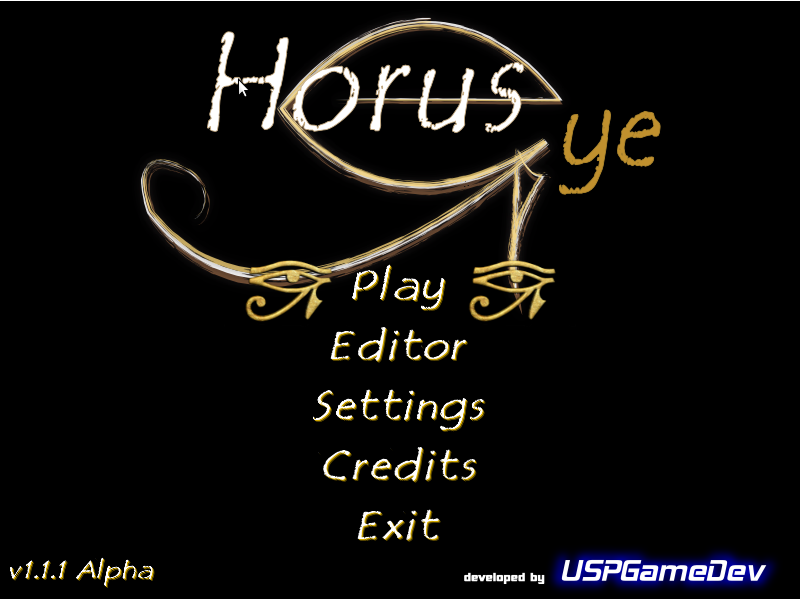
\includegraphics[width=0.6\textwidth]{images/horus_01.png}
%        \caption{Menu do jogo \textit{\textbf{Horus Eye}}}
%        \label{fig:horus_01}
%    \end{figure}
    
%    \begin{wrapfigure}{l}{8cm} % "placement and width parameter for the width of the image space.
%        %\centering
%        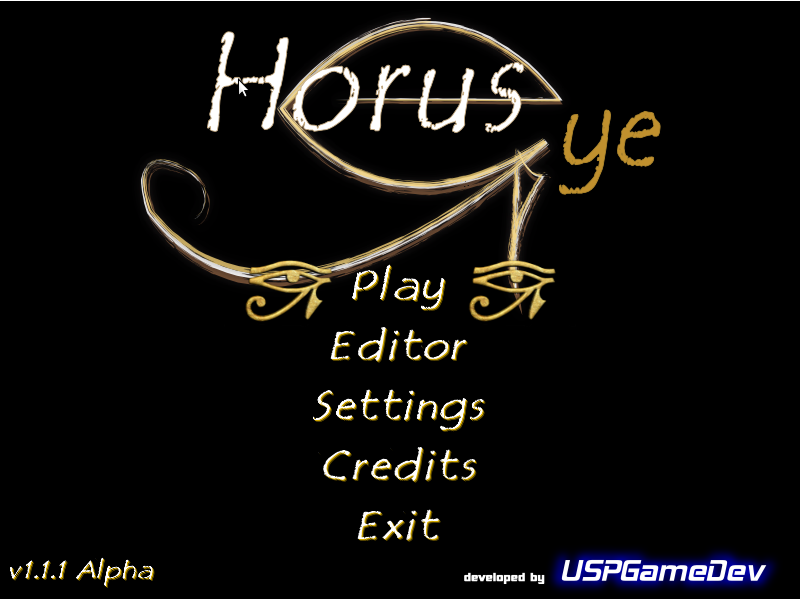
\includegraphics[width=0.6\textwidth]{images/horus_01.png}
%        \caption{Menu do jogo \textit{\textbf{Horus Eye}}}
%        \label{fig:horus_01}
%    \end{wrapfigure}

%    \begin{SCfigure}[0.8][htb]
%        \centering
%        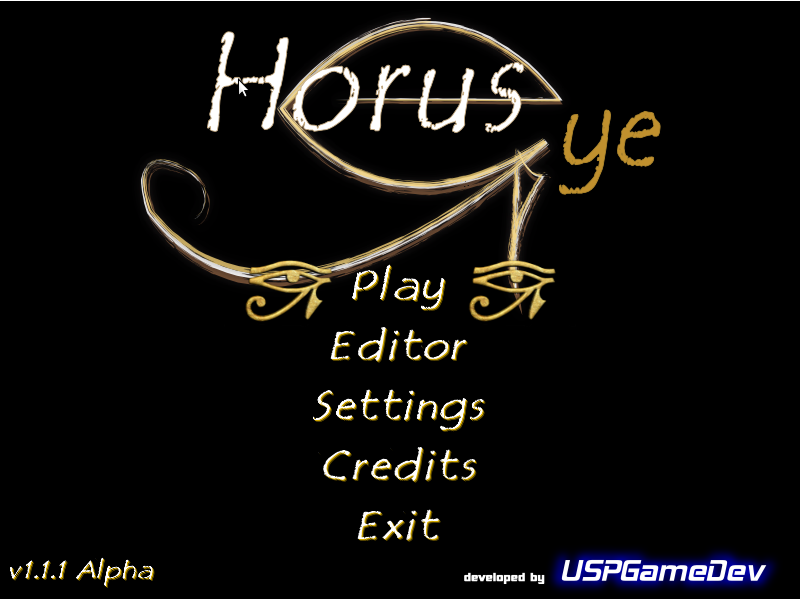
\includegraphics[width=0.6\textwidth]{images/horus_01.png}
%        \caption{ Menu do jogo \textit{\textbf{Horus Eye}} }
%        \label{fig:horus_01}
%    \end{SCfigure}

%\renewcommand{\topfraction}{0.85}
%\renewcommand{\textfraction}{0.1}
%\renewcommand{\floatpagefraction}{0.75}

\clearpage
\section{\LARGE Galeria de Resultados}

    Essa seção foi reservada para exibir imagens, fotos e \textit{screenshots} de diversos
    resultados do USPGameDev, além de alguns \textit{Concept Arts}\footnotemark.
        
    \footnotetext{
        Informações sobre \textit{Concept Art}: \url{http://en.wikipedia.org/wiki/Concept\_art}
    }
    
        \FloatBarrier
        
        %%% Horus Eye %%%
    
        \begin{figure}[htb]
            \centering
            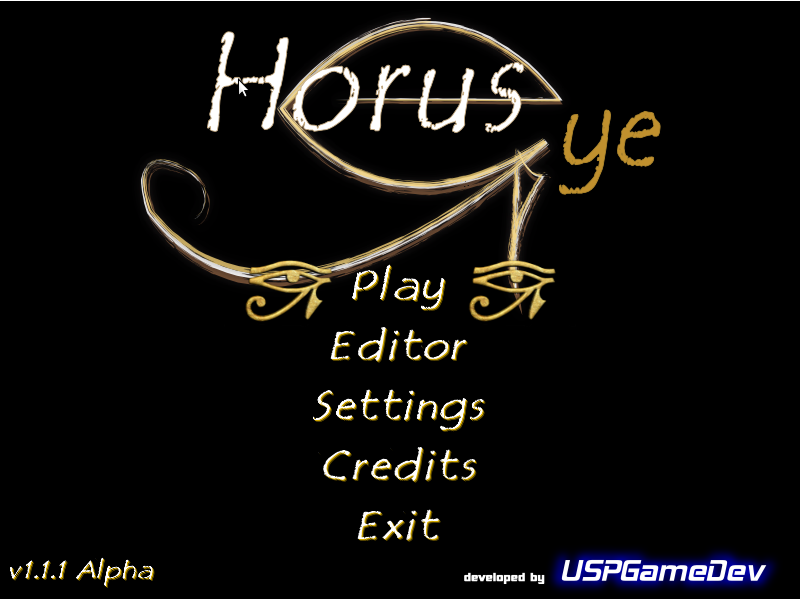
\includegraphics[width=\textwidth]{images/horus_01.png}
            \caption{Menu do jogo \textit{\textbf{Horus Eye}}.}
            \label{fig:horus_01}
        \end{figure}
        
        \begin{figure}[htb]
            \centering
            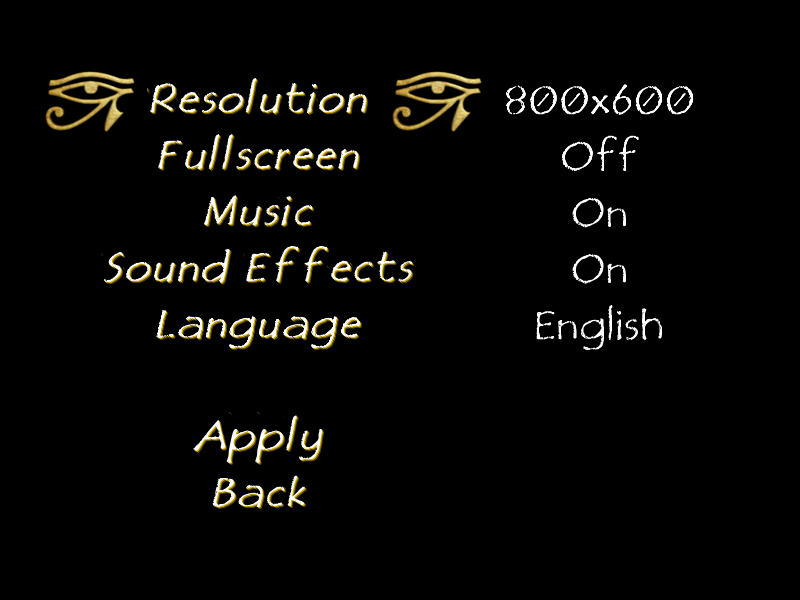
\includegraphics[width=0.9\textwidth]{images/horus_02.png}
            \caption{Cena dentro do jogo \textit{\textbf{Horus Eye}}.}
            \label{fig:horus_02}
        \end{figure}
        
        \begin{figure}[htb]
            \centering
            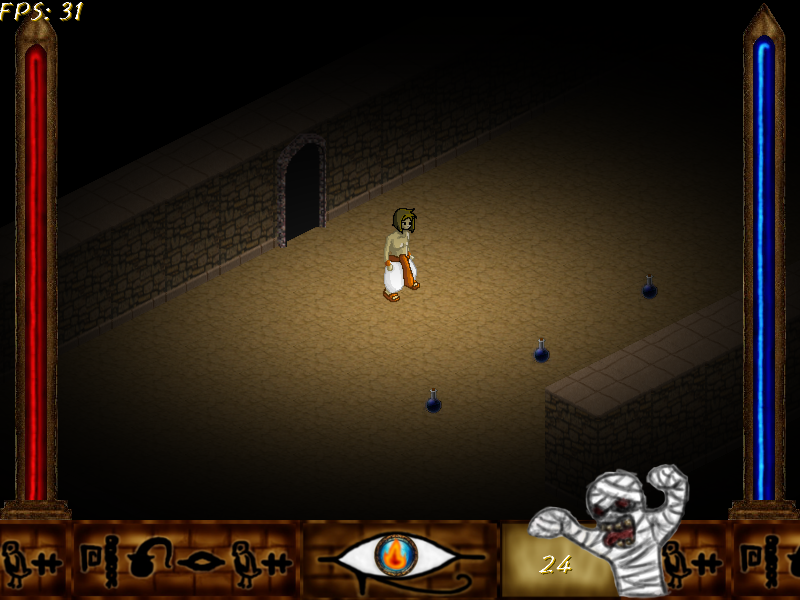
\includegraphics[width=0.9\textwidth]{images/horus_03.png}
            \caption{Inimigos dentro do jogo \textit{\textbf{Horus Eye}}.}
            \label{fig:horus_03}
        \end{figure}
        
        \clearpage
        
        \begin{figure}[htb]
            \centering
            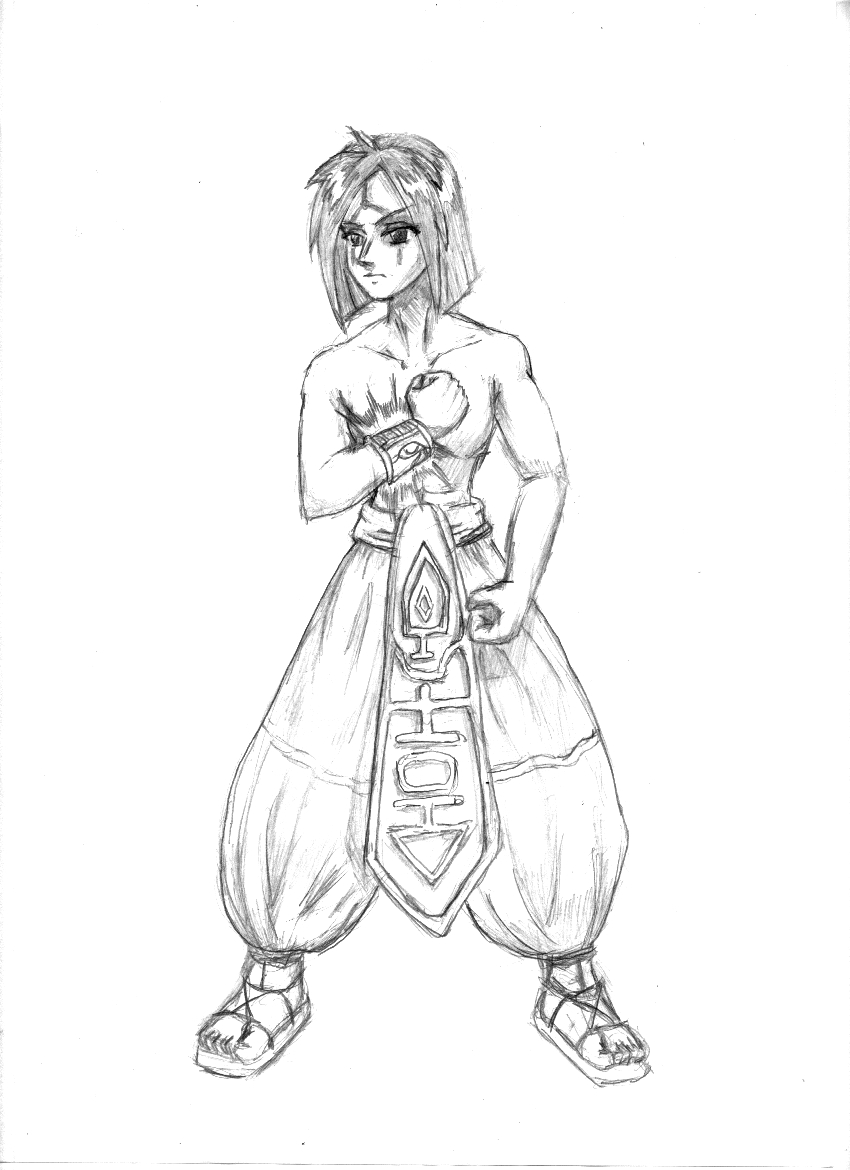
\includegraphics[width=0.9\textwidth]{images/concept_hero.jpg}
            \caption{\textit{Concept Art} do protagonista do jogo \textit{\textbf{Horus Eye}}.}
            \label{fig:concept_01}
        \end{figure}
        
        \begin{figure}[htb]
            \centering
            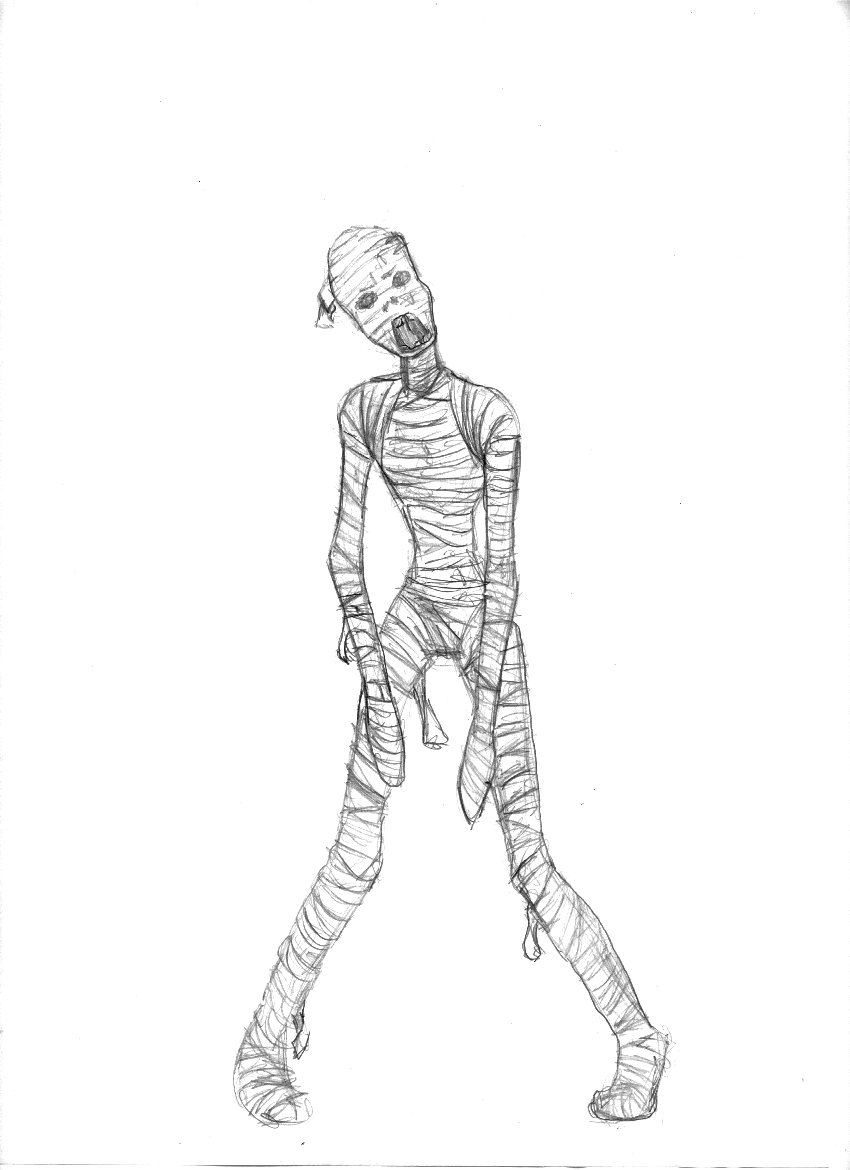
\includegraphics[width=0.9\textwidth]{images/concept_mummy.jpg}
            \caption{\textit{Concept Art} dos monstros do jogo \textit{\textbf{Horus Eye}}.}
            \label{fig:concept_02}
        \end{figure}
        
        \begin{figure}[htb]
            \centering
            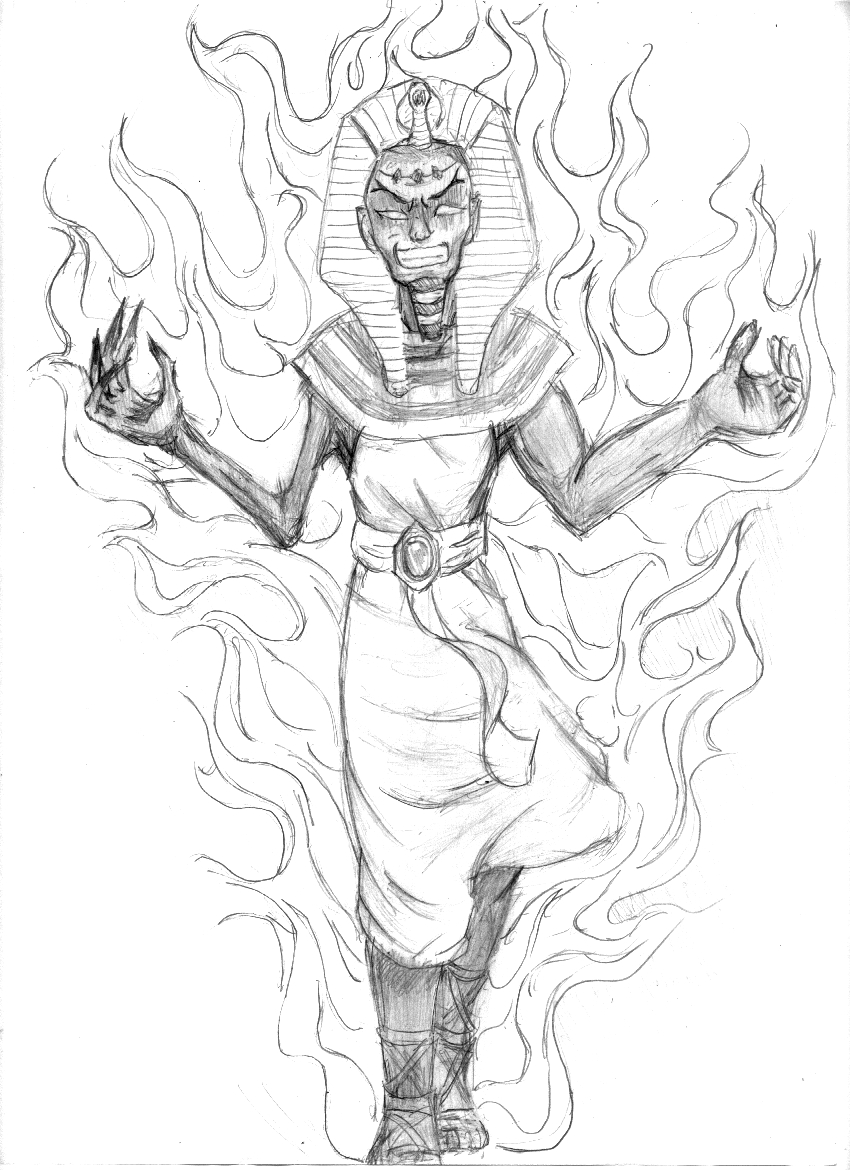
\includegraphics[width=0.9\textwidth]{images/concept_pharaoh.jpg}
            \caption{\textit{Concept Art} do vilão do jogo \textit{\textbf{Horus Eye}}.}
            \label{fig:concept_03}
        \end{figure}
        
        %%% Pirates %%%
    
        \begin{figure}[htb]
            \centering
            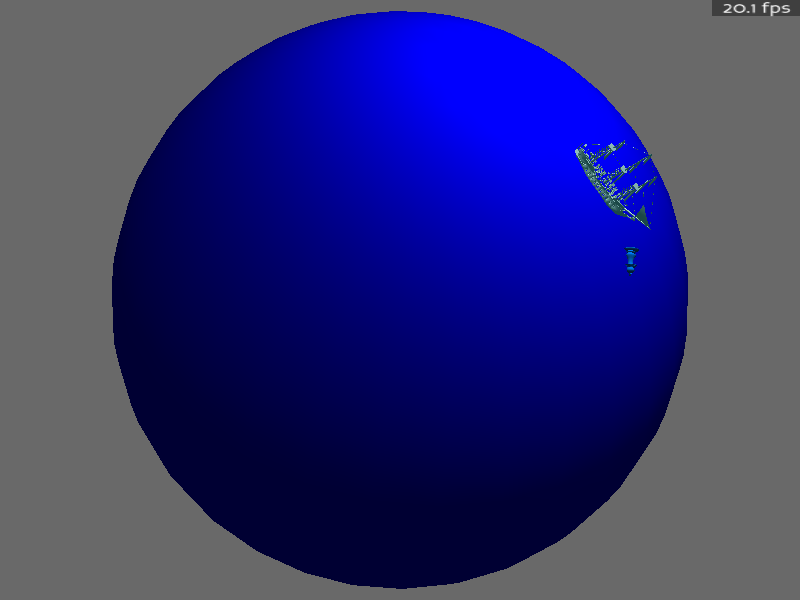
\includegraphics[width=0.9\textwidth]{images/pirates_01.png}
            \caption{Estágio atual do desenvolvimento do \textit{\textbf{Pirates}}.}
            \label{fig:pirates_01}
        \end{figure}
    
        \begin{figure}[htb]
            \centering
            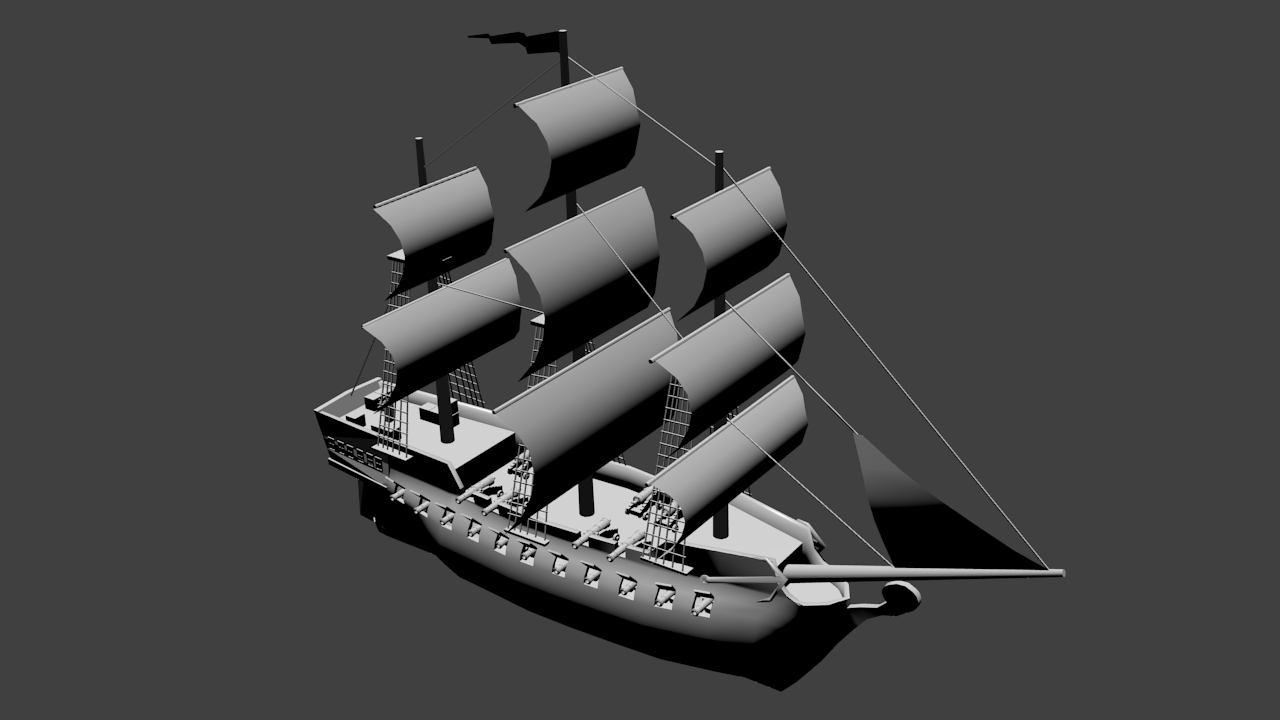
\includegraphics[width=0.9\textwidth]{images/pirates_02.png}
            \caption{Modelo tridimensional feito para o jogo \textit{\textbf{Pirates}}.}
            \label{fig:pirates_02}
        \end{figure}
        
        %%% Palestras %%%
        
        \begin{figure}[htb]
            \centering
            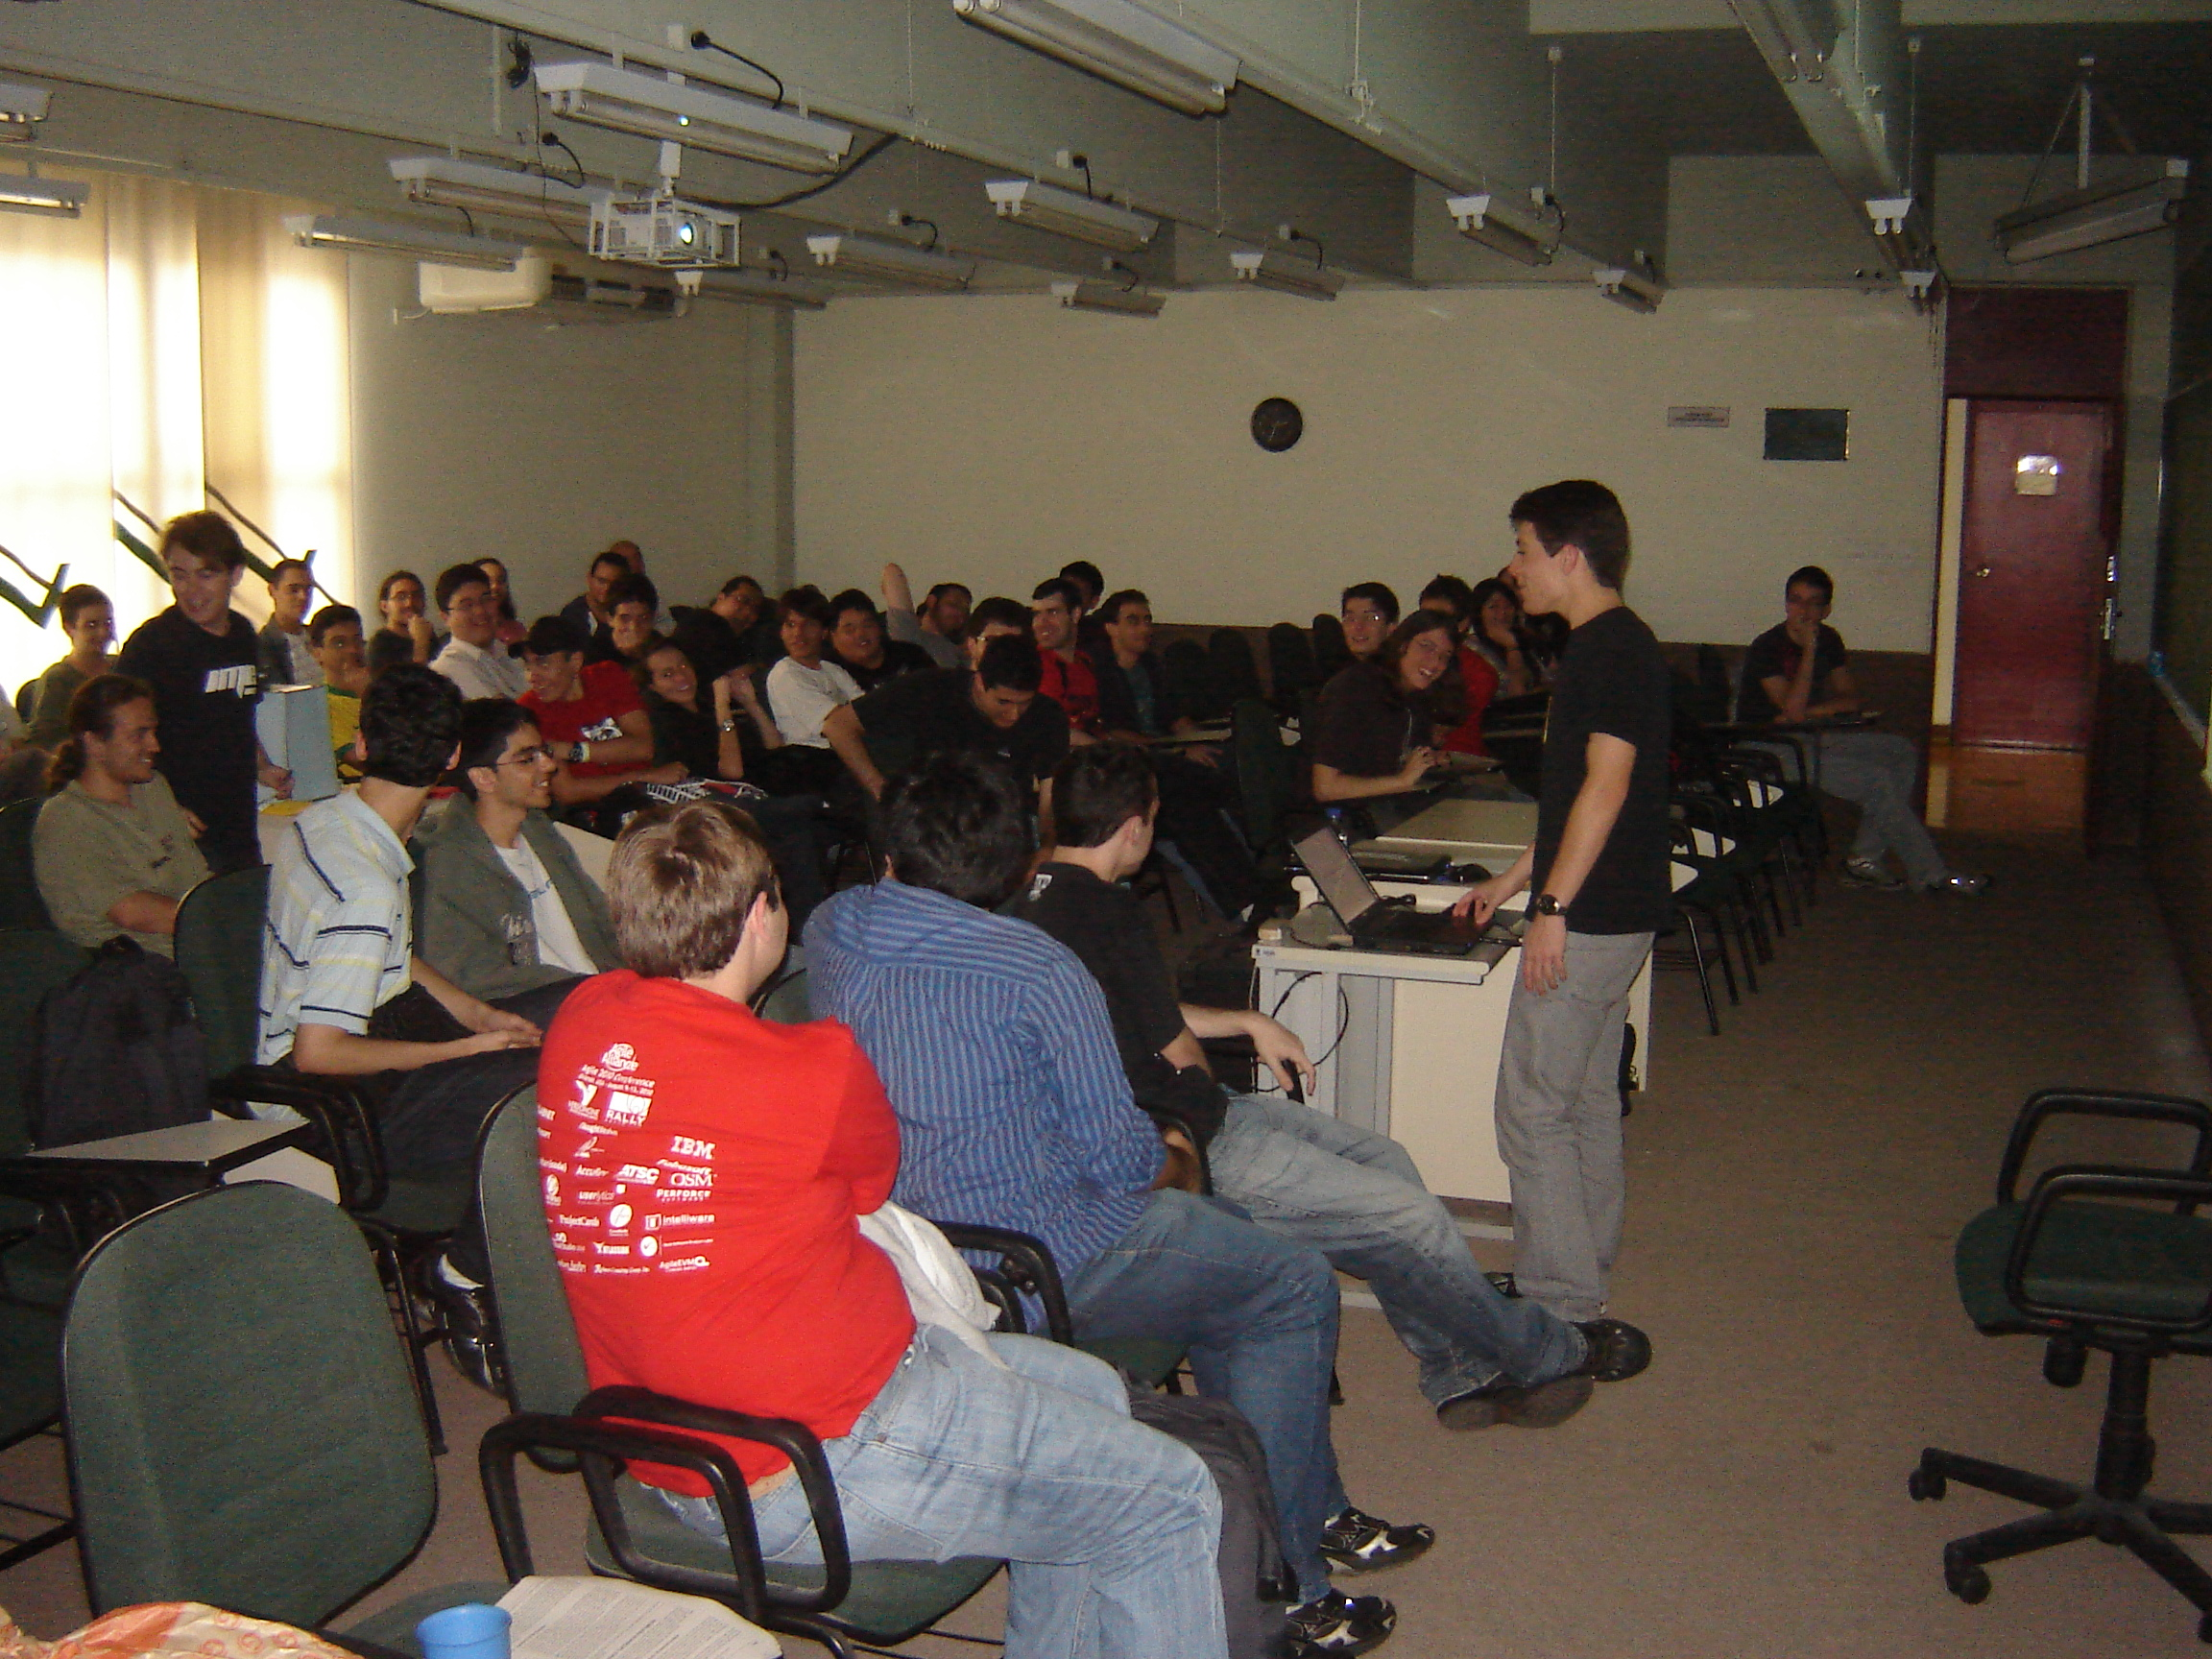
\includegraphics[width=0.9\textwidth]{images/palestra_01.jpg}
            \caption{Palestra do USPGameDev, na qual o \textit{\textbf{Horus Eye}} foi lançado}
            \label{fig:palestra_01}
        \end{figure}
        
        \begin{figure}[htb]
            \centering
            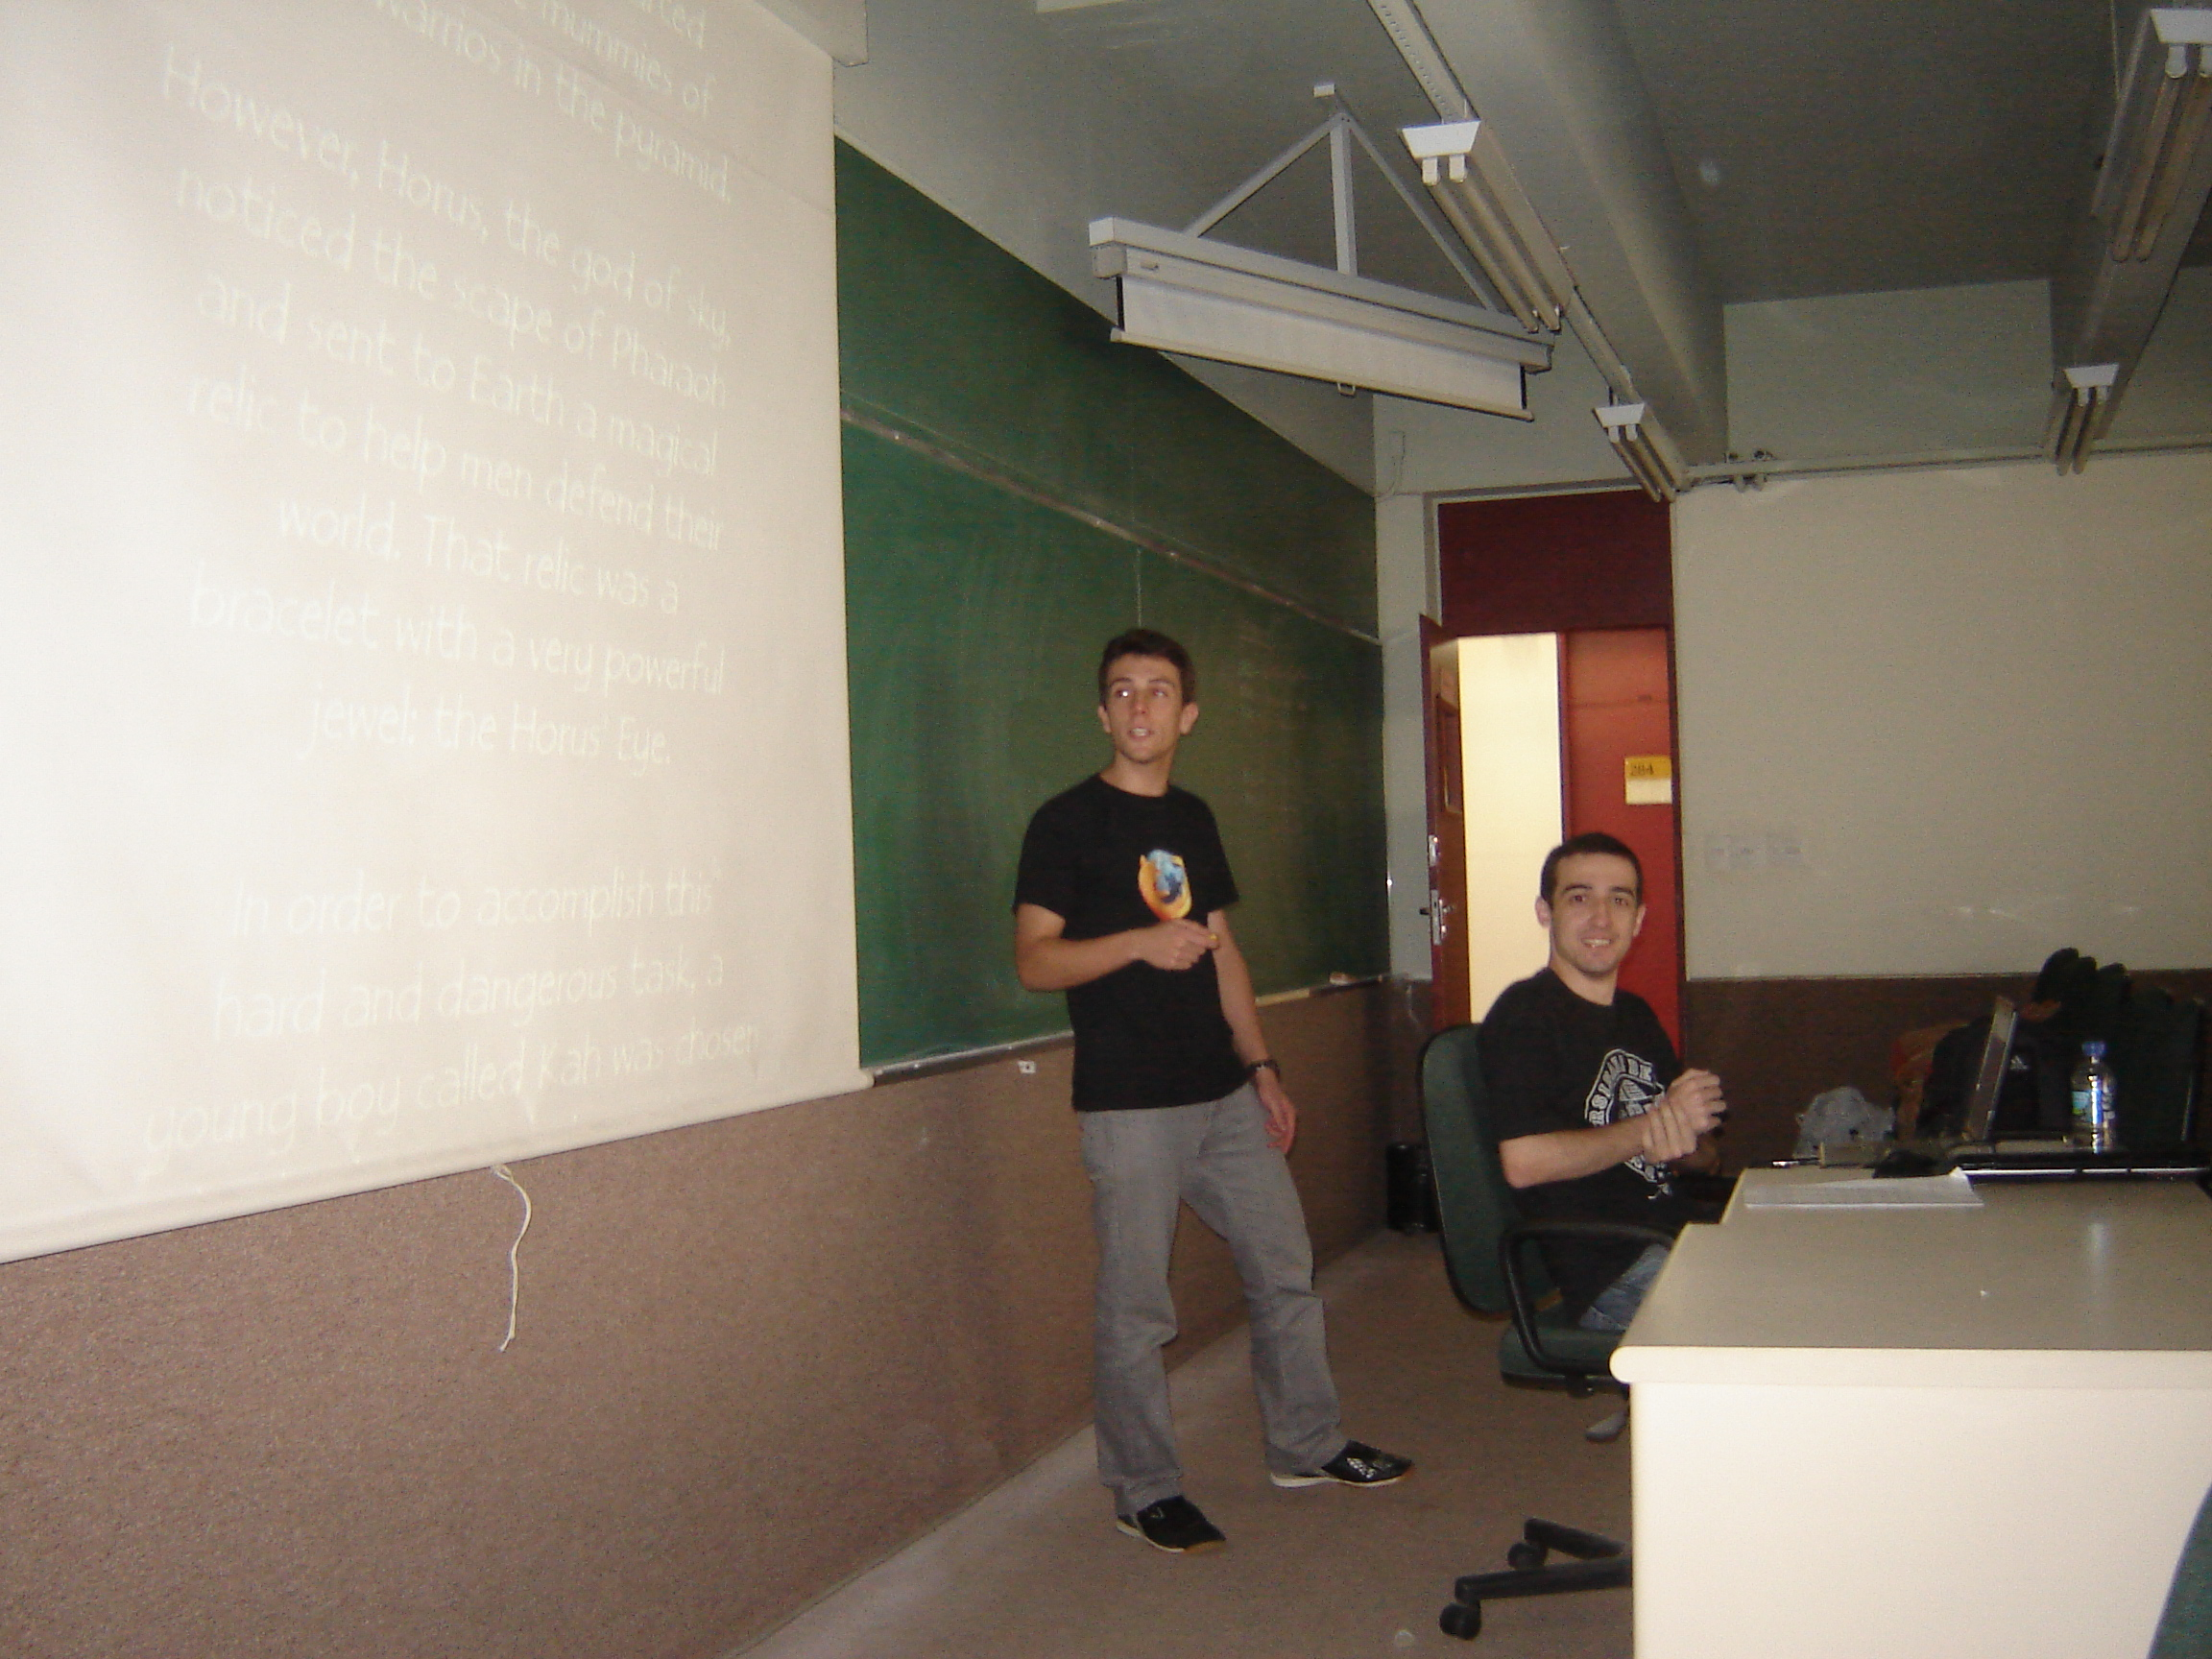
\includegraphics[width=0.9\textwidth]{images/palestra_02.jpg}
            \caption{Demonstração do \textit{\textbf{Horus Eye}} durante a palestra.}
            \label{fig:palestra_02}
        \end{figure}
        
        \begin{figure}[htb]
            \centering
            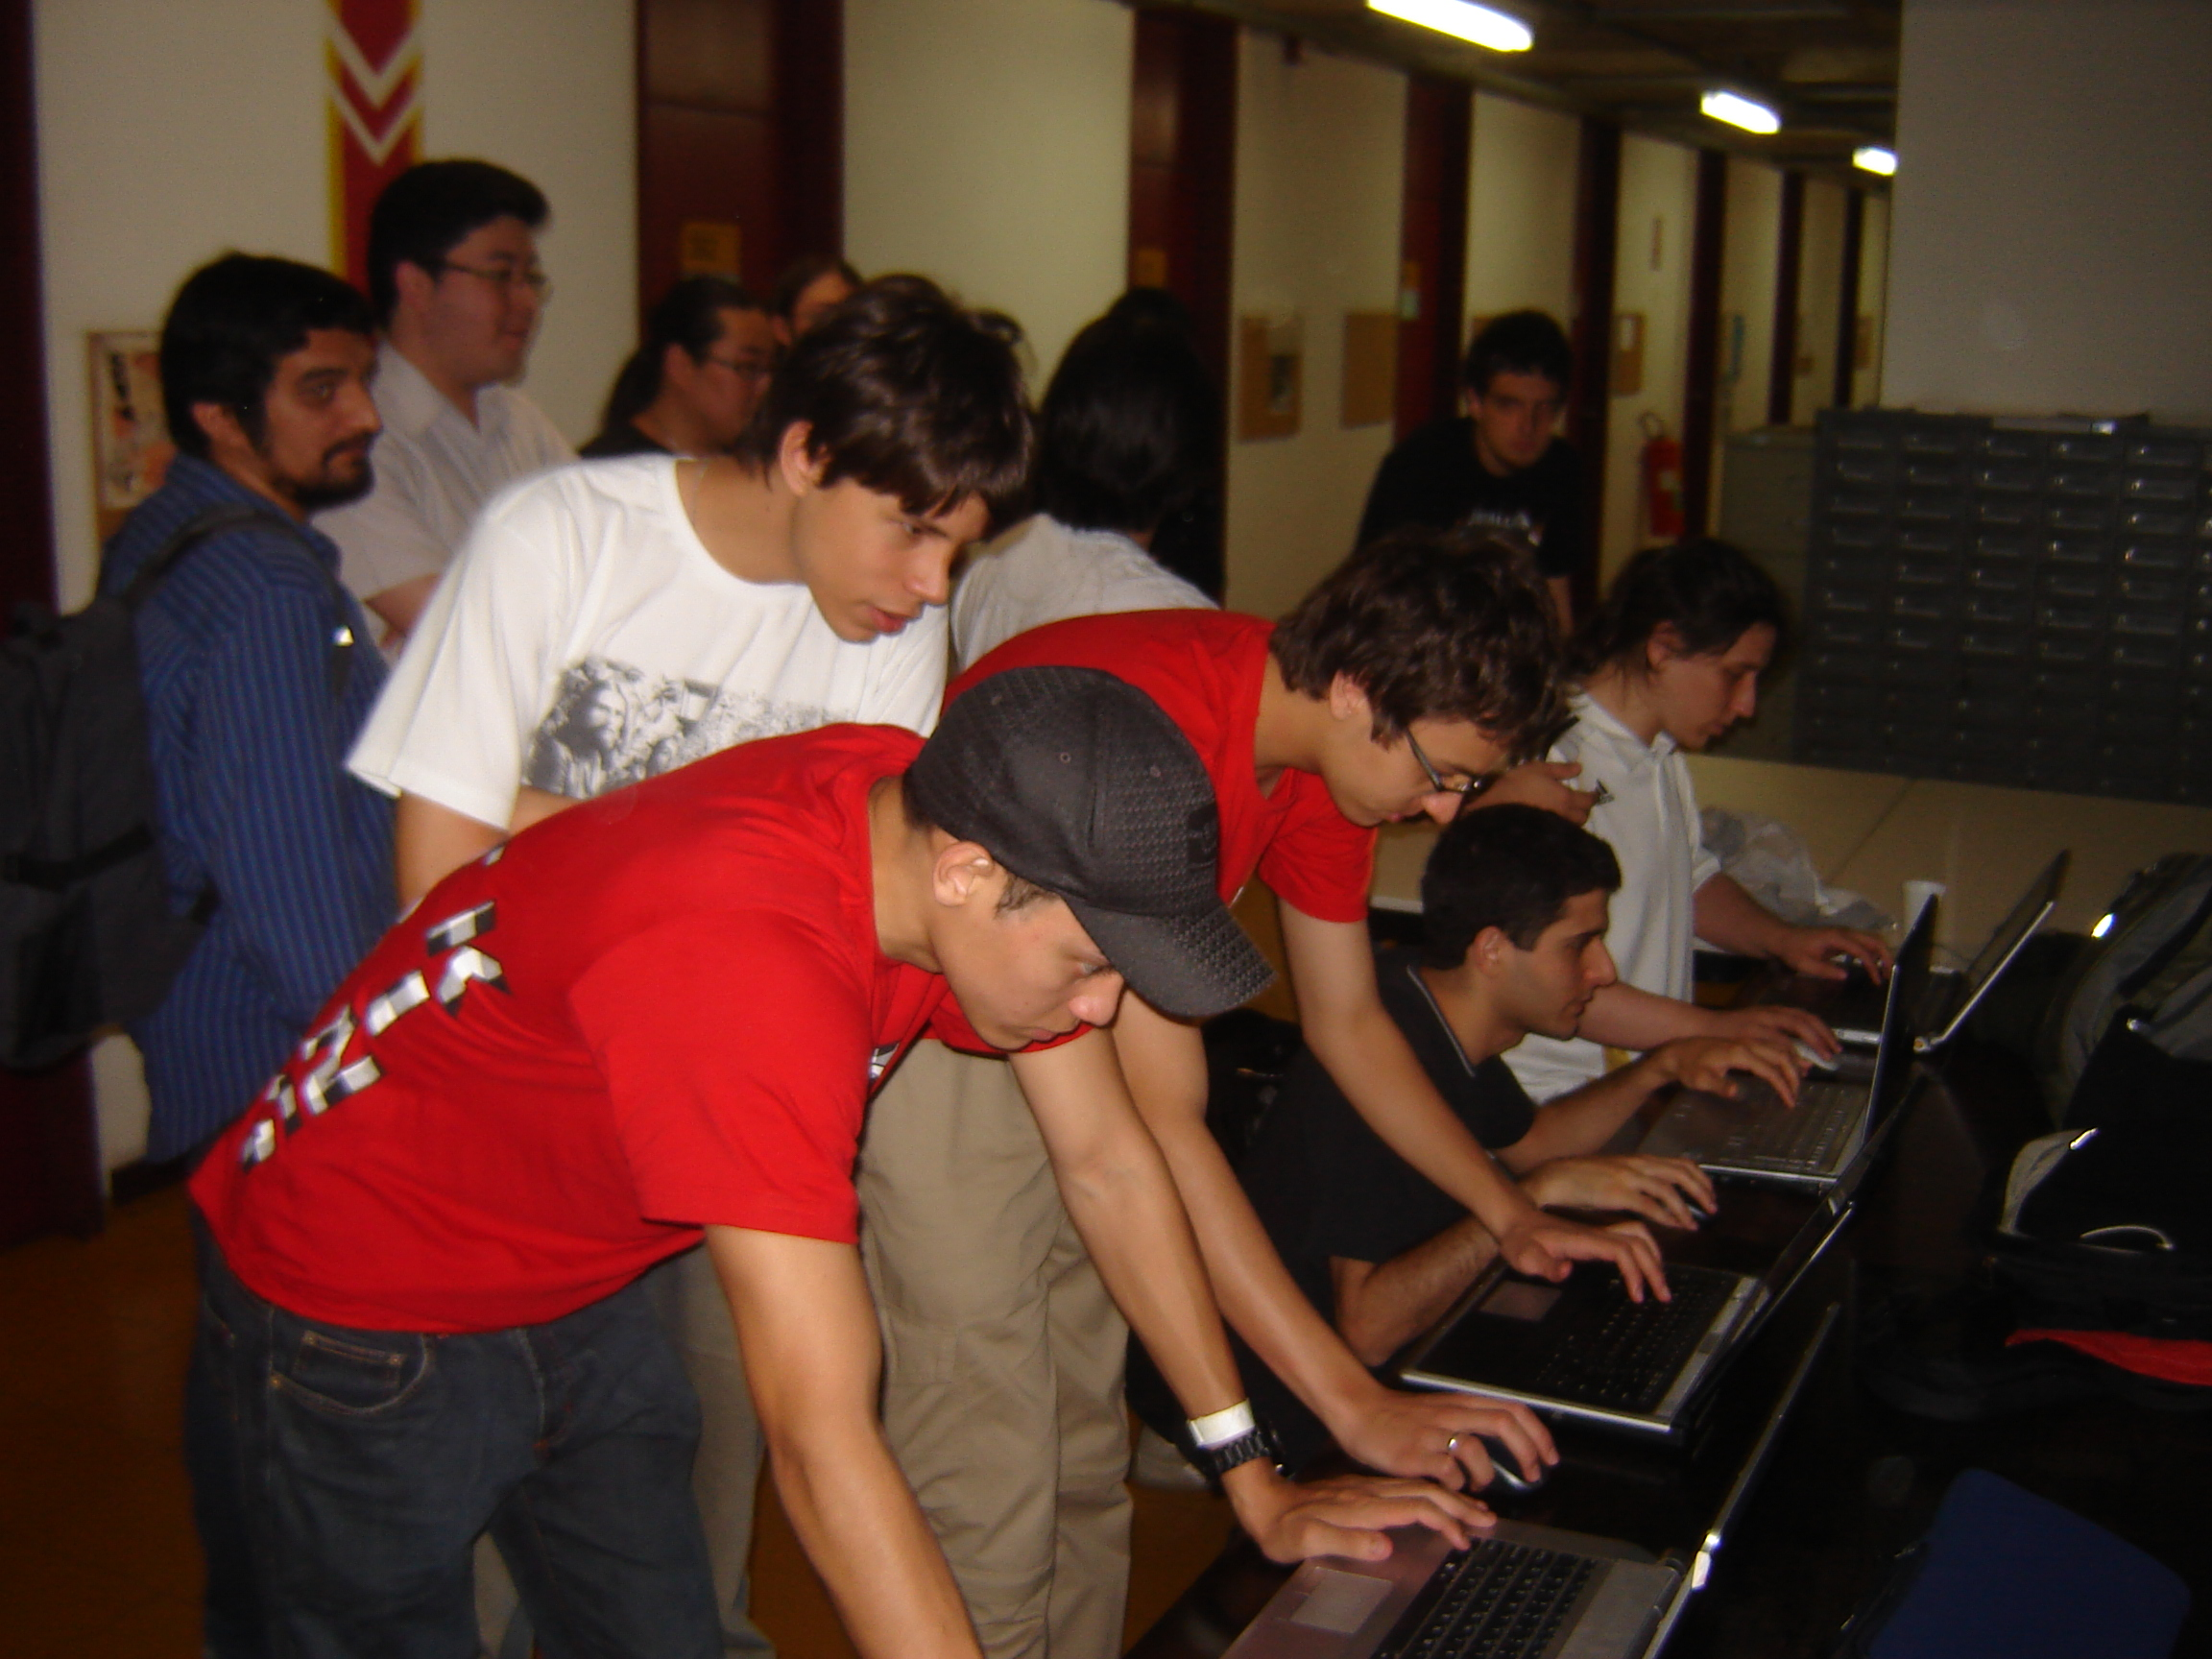
\includegraphics[width=0.9\textwidth]{images/palestra_03.jpg}
            \caption{Participantes da palestra testando o \textit{\textbf{Horus Eye}}.}
            \label{fig:palestra_03}
        \end{figure}
        
        %%% Processo seletivo %%%
        
        \begin{figure}[htb]
            \centering
            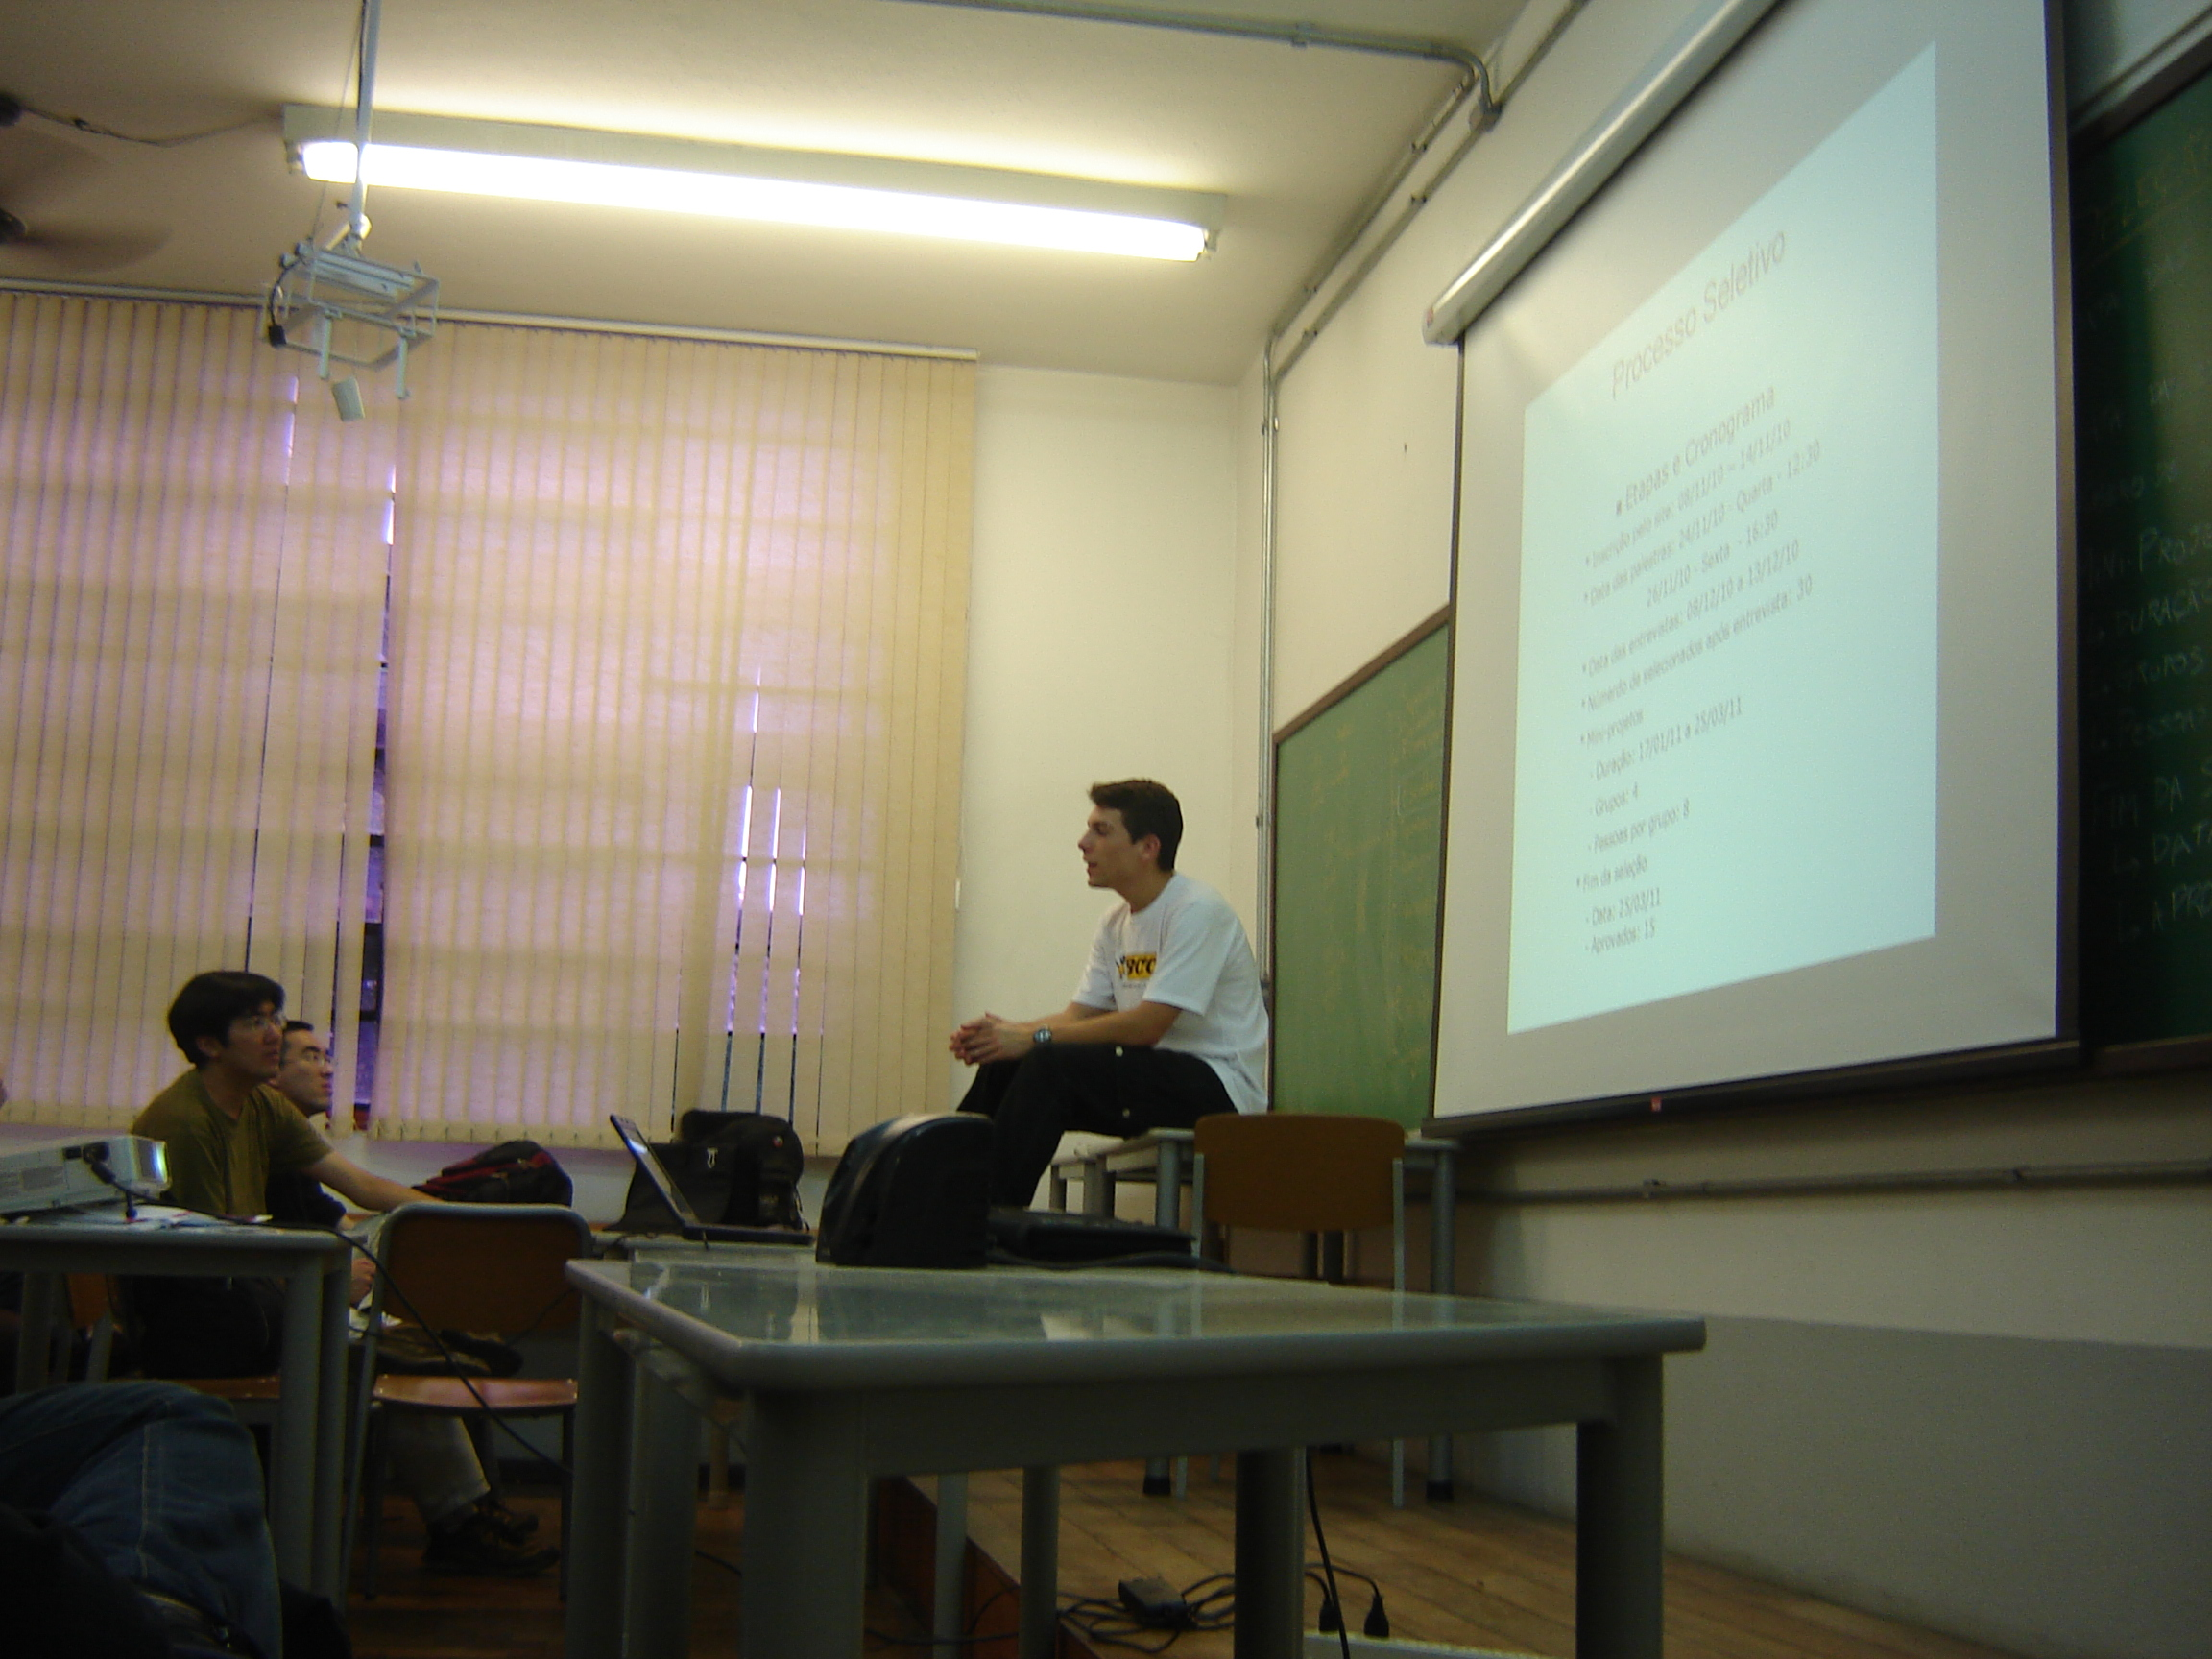
\includegraphics[width=0.9\textwidth]{images/seletivo_01.jpg}
            \caption{Apresentação de abertura do processo seletivo.}
            \label{fig:seletivo_01}
        \end{figure}
        
        \begin{figure}[htb]
            \centering
            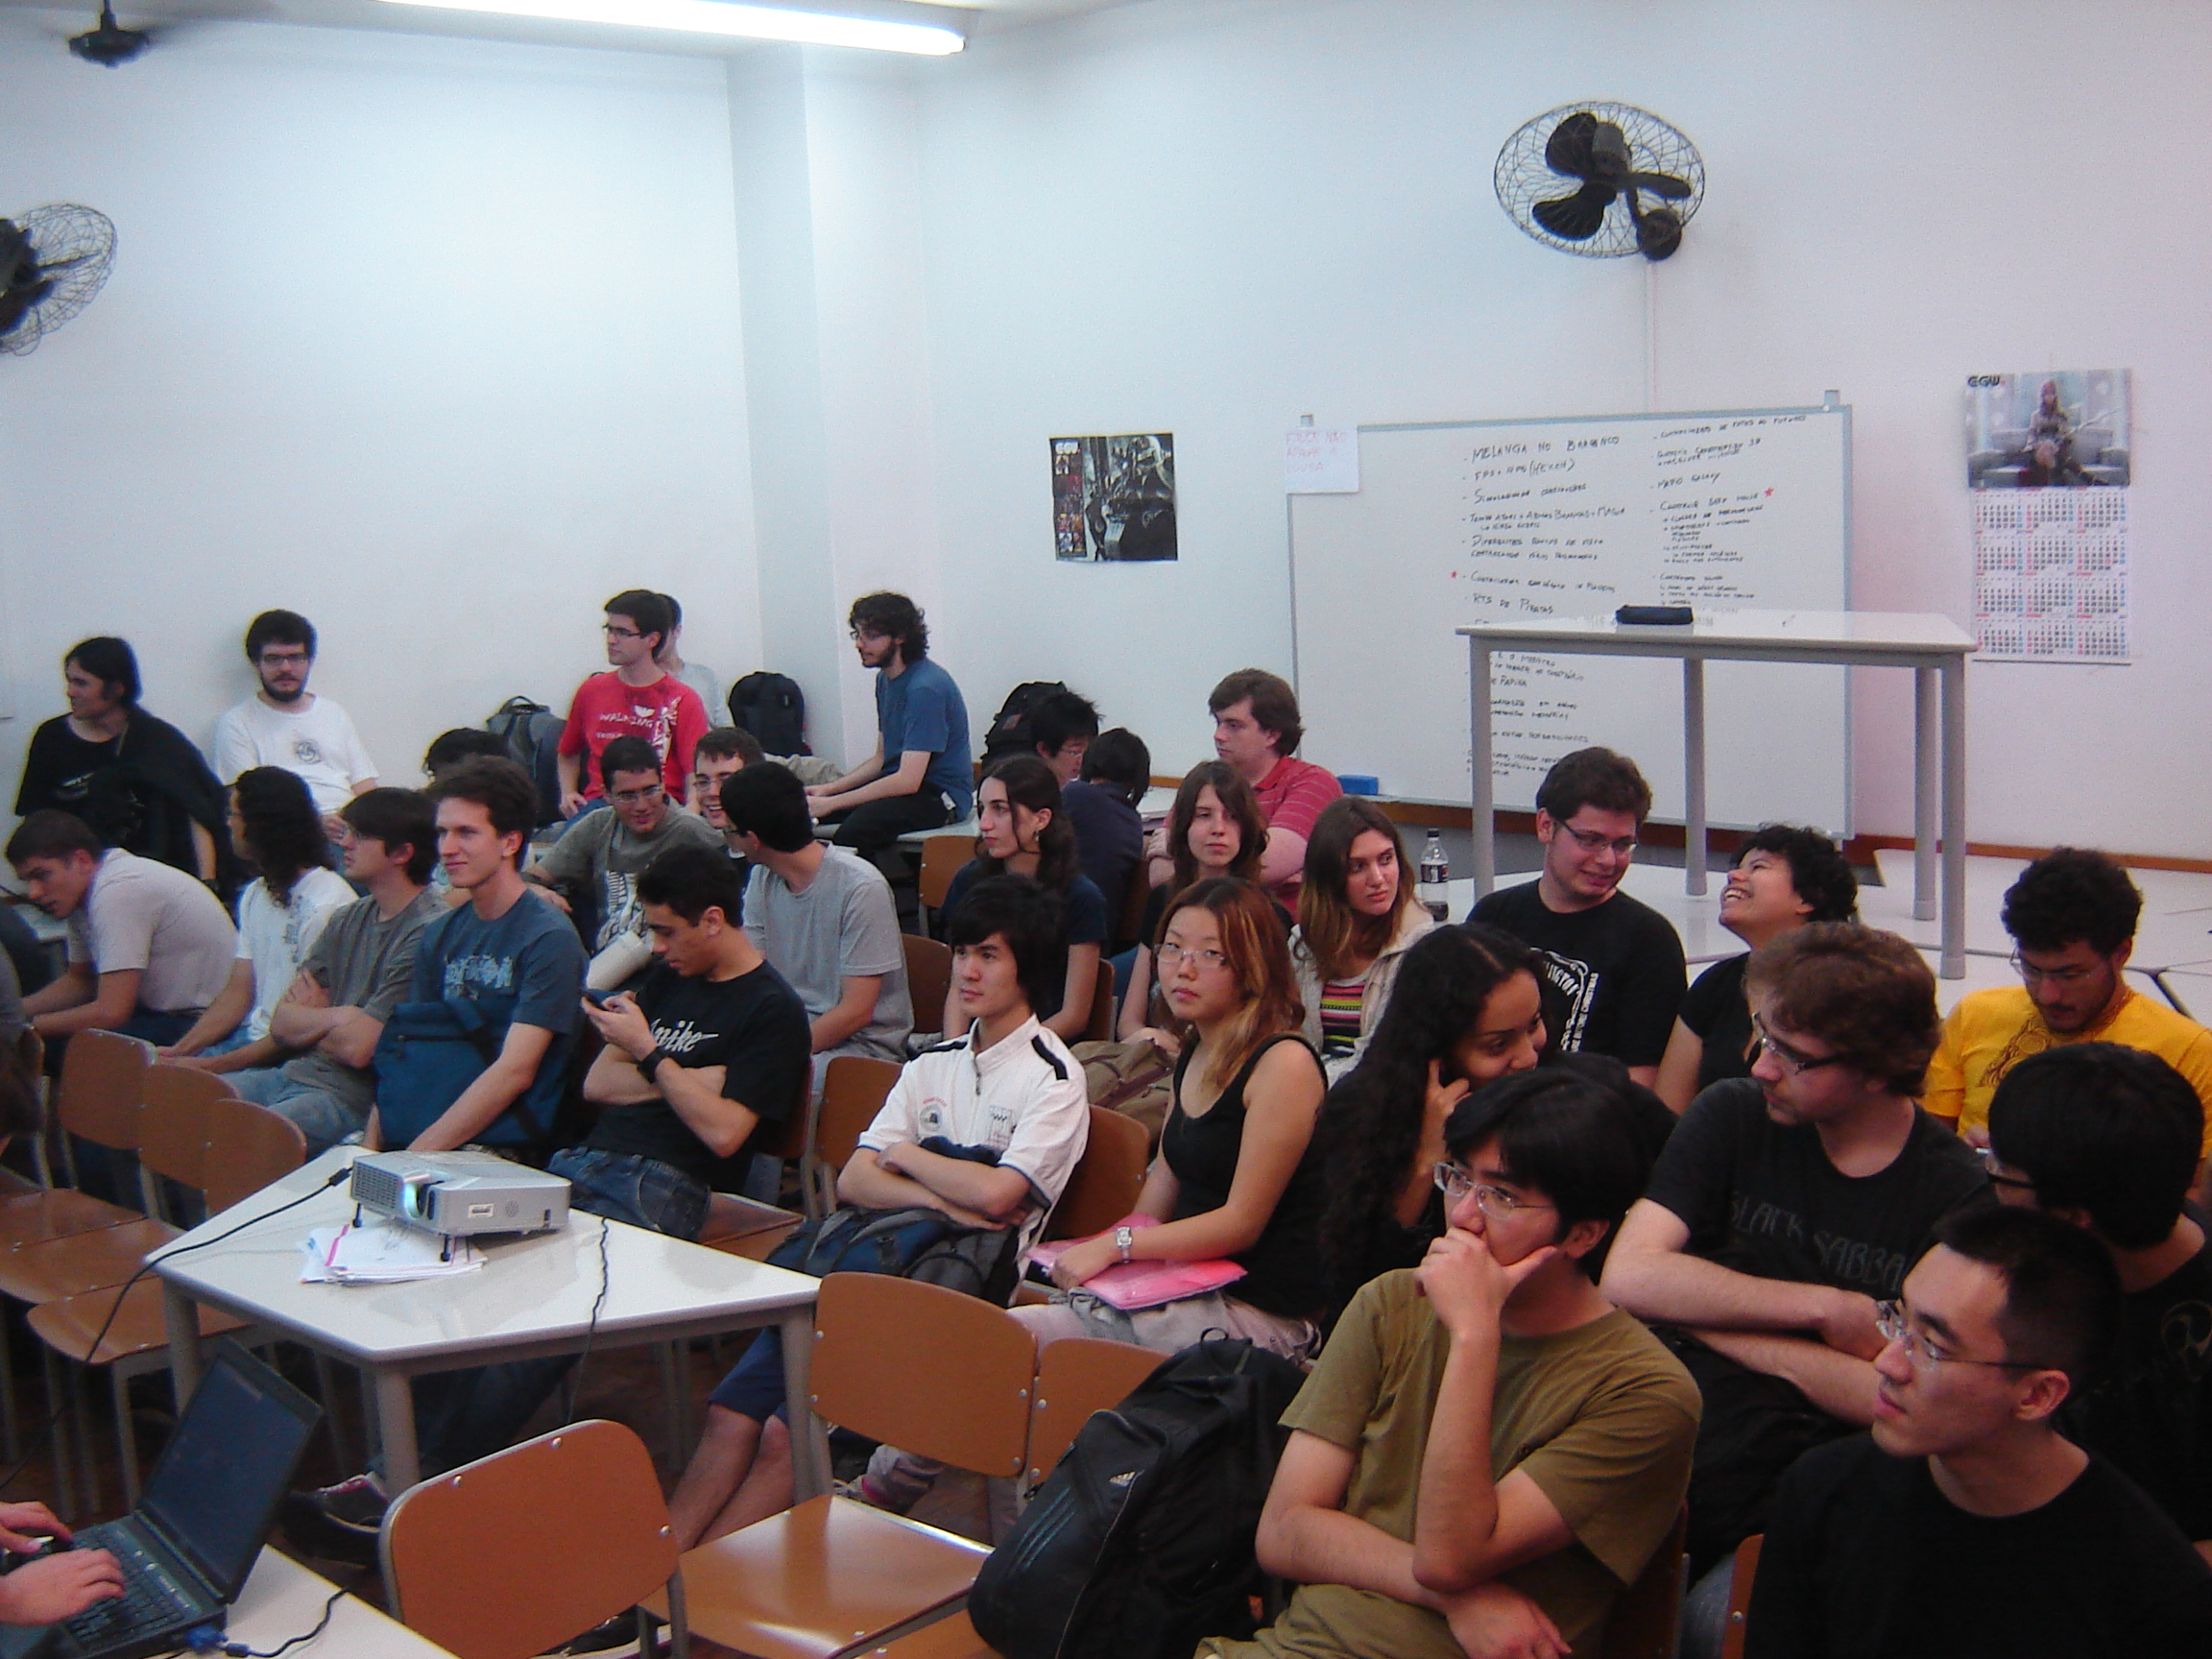
\includegraphics[width=0.9\textwidth]{images/seletivo_02.jpg}
            \caption{Participantes do processo seletivo.}
            \label{fig:seletivo_02}
        \end{figure}
        
        %%% Site %%%
        
        \begin{figure}[htb]
            \centering
            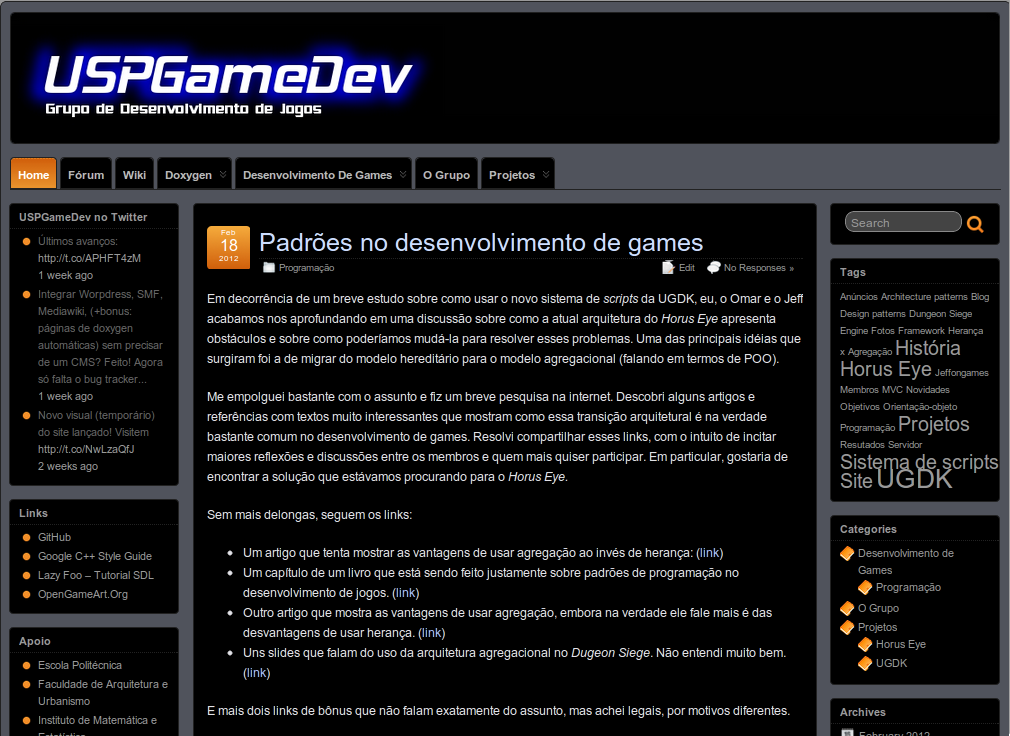
\includegraphics[width=0.9\textwidth]{images/site_01.png}
            \caption{O novo site do USPGameDev.}
            \label{fig:site_01}
        \end{figure}
        
        \begin{figure}[htb]
            \centering
            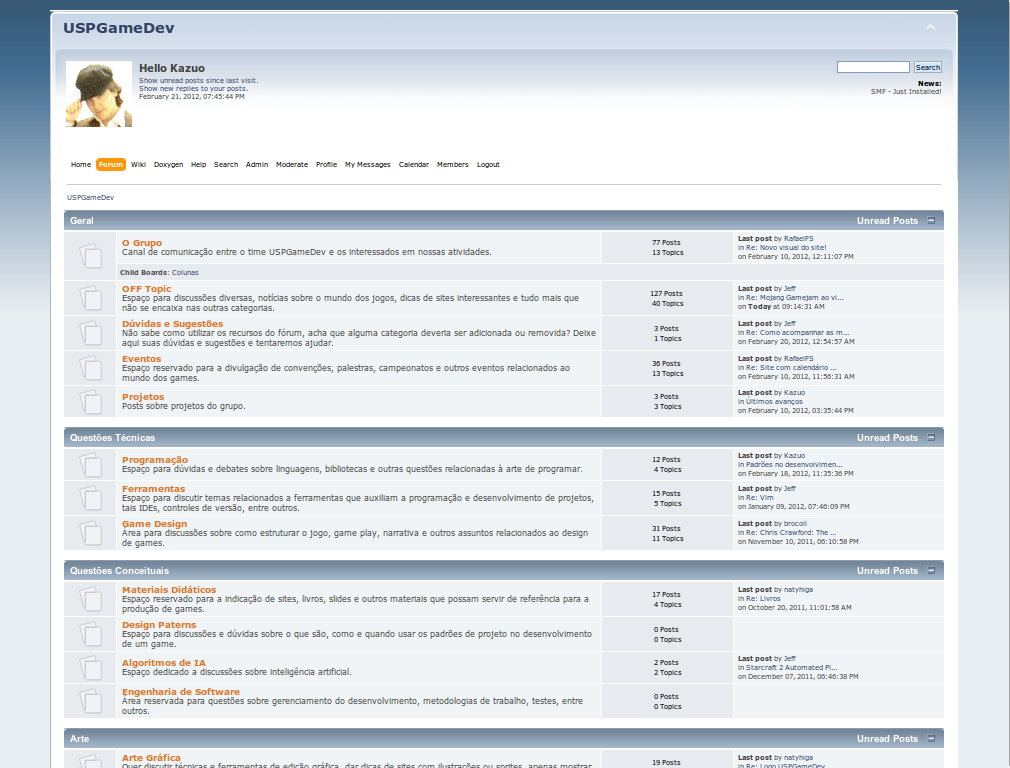
\includegraphics[width=0.85\textwidth]{images/site_02.png}
            \caption{Fórum do USPGameDev.}
            \label{fig:site_02}
        \end{figure}
        
        \begin{figure}[htb]
            \centering
            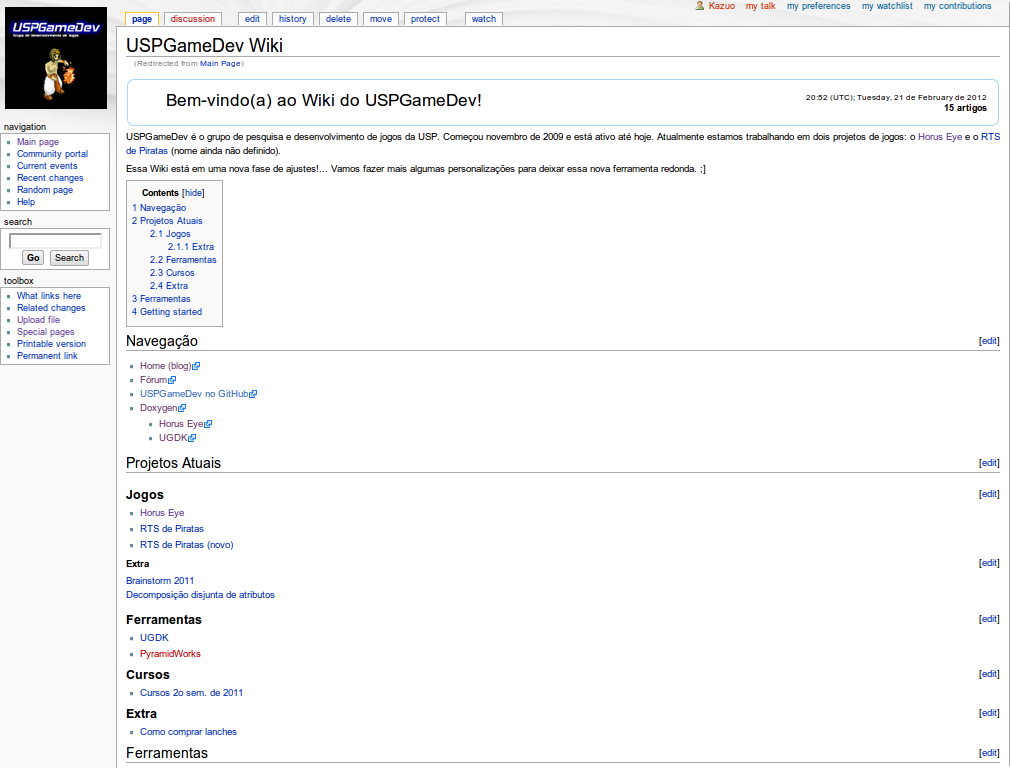
\includegraphics[width=0.85\textwidth]{images/site_03.png}
            \caption{Wiki do USPGameDev.}
            \label{fig:site_03}
        \end{figure}
        
        \clearpage
        
        \begin{figure}[htb]
            \centering
            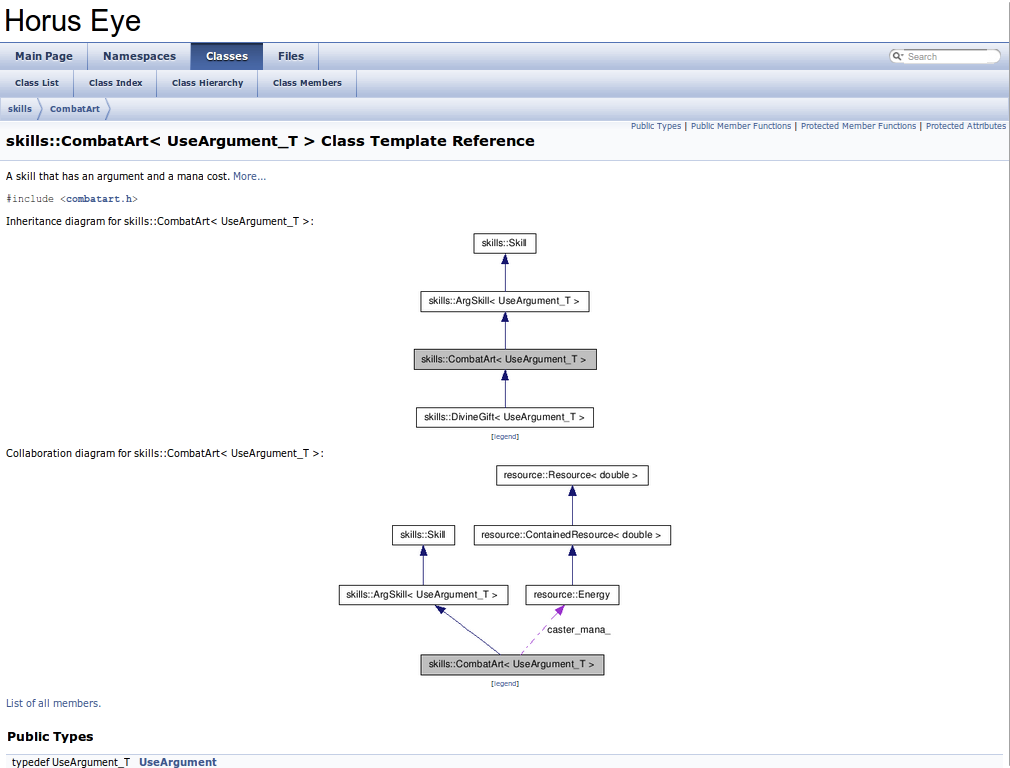
\includegraphics[width=0.85\textwidth]{images/site_04.png}
            \caption{Documentação \textit{on-line} do \textit{\textbf{Horus Eye}}.}
            \label{fig:site_04}
        \end{figure}
    
    %\subsection{Imagens sobre o jogo \textit{\textbf{Horus Eye}}}
        
        %\FloatBarrier
        
        %\FloatBarrier
    
    %\subsection{Imagens sobre o jogo \textit{Pirates}}
    
        %\FloatBarrier
        
        %\FloatBarrier
    
    %\subsection{Imagens do site}
    
        %\FloatBarrier
        
        %\FloatBarrier
        
    %\subsection{Imagens das palestras}
    
        %\FloatBarrier
        
        %\FloatBarrier
        
    %\subsection{Imagens do processo seletivo}
    
        %\FloatBarrier
        
        %\FloatBarrier

\section{\LARGE Observações bibliográficas}

    Todas as referências usadas nesse relatório têm sua bibliografia citada na página em que são
    usadas e/ou mencionadas pela primeira vez. Caso contrário, a referência é proveniente do próprio
    USPGameDev, o que significa que pode ser encontrada no site oficial, salvo o caso do
    \textit{Game Design Document}, que está devidamente explicado na seção em que aparece.
    
    As imagens também são todas provenientes dos materiais do próprio grupo, sejam elas fotos,
    \textit{screenshots}, ou \textit{Concept Arts}.

% End of document.
\end{document}

